% Options for packages loaded elsewhere
\PassOptionsToPackage{unicode}{hyperref}
\PassOptionsToPackage{hyphens}{url}
\PassOptionsToPackage{dvipsnames,svgnames,x11names}{xcolor}
%
\documentclass[
  a4paper,
]{ltjsbook}

\usepackage{amsmath,amssymb}
\usepackage{iftex}
\ifPDFTeX
  \usepackage[T1]{fontenc}
  \usepackage[utf8]{inputenc}
  \usepackage{textcomp} % provide euro and other symbols
\else % if luatex or xetex
  \usepackage{unicode-math}
  \defaultfontfeatures{Scale=MatchLowercase}
  \defaultfontfeatures[\rmfamily]{Ligatures=TeX,Scale=1}
\fi
\usepackage{lmodern}
\ifPDFTeX\else  
    % xetex/luatex font selection
\fi
% Use upquote if available, for straight quotes in verbatim environments
\IfFileExists{upquote.sty}{\usepackage{upquote}}{}
\IfFileExists{microtype.sty}{% use microtype if available
  \usepackage[]{microtype}
  \UseMicrotypeSet[protrusion]{basicmath} % disable protrusion for tt fonts
}{}
\makeatletter
\@ifundefined{KOMAClassName}{% if non-KOMA class
  \IfFileExists{parskip.sty}{%
    \usepackage{parskip}
  }{% else
    \setlength{\parindent}{0pt}
    \setlength{\parskip}{6pt plus 2pt minus 1pt}}
}{% if KOMA class
  \KOMAoptions{parskip=half}}
\makeatother
\usepackage{xcolor}
\usepackage[top=30mm,left=20mm,heightrounded]{geometry}
\ifLuaTeX
  \usepackage{luacolor}
  \usepackage[soul]{lua-ul}
\else
  \usepackage{soul}
  
\fi
\setlength{\emergencystretch}{3em} % prevent overfull lines
\setcounter{secnumdepth}{5}
% Make \paragraph and \subparagraph free-standing
\makeatletter
\ifx\paragraph\undefined\else
  \let\oldparagraph\paragraph
  \renewcommand{\paragraph}{
    \@ifstar
      \xxxParagraphStar
      \xxxParagraphNoStar
  }
  \newcommand{\xxxParagraphStar}[1]{\oldparagraph*{#1}\mbox{}}
  \newcommand{\xxxParagraphNoStar}[1]{\oldparagraph{#1}\mbox{}}
\fi
\ifx\subparagraph\undefined\else
  \let\oldsubparagraph\subparagraph
  \renewcommand{\subparagraph}{
    \@ifstar
      \xxxSubParagraphStar
      \xxxSubParagraphNoStar
  }
  \newcommand{\xxxSubParagraphStar}[1]{\oldsubparagraph*{#1}\mbox{}}
  \newcommand{\xxxSubParagraphNoStar}[1]{\oldsubparagraph{#1}\mbox{}}
\fi
\makeatother

\usepackage{color}
\usepackage{fancyvrb}
\newcommand{\VerbBar}{|}
\newcommand{\VERB}{\Verb[commandchars=\\\{\}]}
\DefineVerbatimEnvironment{Highlighting}{Verbatim}{commandchars=\\\{\}}
% Add ',fontsize=\small' for more characters per line
\usepackage{framed}
\definecolor{shadecolor}{RGB}{241,243,245}
\newenvironment{Shaded}{\begin{snugshade}}{\end{snugshade}}
\newcommand{\AlertTok}[1]{\textcolor[rgb]{0.68,0.00,0.00}{#1}}
\newcommand{\AnnotationTok}[1]{\textcolor[rgb]{0.37,0.37,0.37}{#1}}
\newcommand{\AttributeTok}[1]{\textcolor[rgb]{0.40,0.45,0.13}{#1}}
\newcommand{\BaseNTok}[1]{\textcolor[rgb]{0.68,0.00,0.00}{#1}}
\newcommand{\BuiltInTok}[1]{\textcolor[rgb]{0.00,0.23,0.31}{#1}}
\newcommand{\CharTok}[1]{\textcolor[rgb]{0.13,0.47,0.30}{#1}}
\newcommand{\CommentTok}[1]{\textcolor[rgb]{0.37,0.37,0.37}{#1}}
\newcommand{\CommentVarTok}[1]{\textcolor[rgb]{0.37,0.37,0.37}{\textit{#1}}}
\newcommand{\ConstantTok}[1]{\textcolor[rgb]{0.56,0.35,0.01}{#1}}
\newcommand{\ControlFlowTok}[1]{\textcolor[rgb]{0.00,0.23,0.31}{\textbf{#1}}}
\newcommand{\DataTypeTok}[1]{\textcolor[rgb]{0.68,0.00,0.00}{#1}}
\newcommand{\DecValTok}[1]{\textcolor[rgb]{0.68,0.00,0.00}{#1}}
\newcommand{\DocumentationTok}[1]{\textcolor[rgb]{0.37,0.37,0.37}{\textit{#1}}}
\newcommand{\ErrorTok}[1]{\textcolor[rgb]{0.68,0.00,0.00}{#1}}
\newcommand{\ExtensionTok}[1]{\textcolor[rgb]{0.00,0.23,0.31}{#1}}
\newcommand{\FloatTok}[1]{\textcolor[rgb]{0.68,0.00,0.00}{#1}}
\newcommand{\FunctionTok}[1]{\textcolor[rgb]{0.28,0.35,0.67}{#1}}
\newcommand{\ImportTok}[1]{\textcolor[rgb]{0.00,0.46,0.62}{#1}}
\newcommand{\InformationTok}[1]{\textcolor[rgb]{0.37,0.37,0.37}{#1}}
\newcommand{\KeywordTok}[1]{\textcolor[rgb]{0.00,0.23,0.31}{\textbf{#1}}}
\newcommand{\NormalTok}[1]{\textcolor[rgb]{0.00,0.23,0.31}{#1}}
\newcommand{\OperatorTok}[1]{\textcolor[rgb]{0.37,0.37,0.37}{#1}}
\newcommand{\OtherTok}[1]{\textcolor[rgb]{0.00,0.23,0.31}{#1}}
\newcommand{\PreprocessorTok}[1]{\textcolor[rgb]{0.68,0.00,0.00}{#1}}
\newcommand{\RegionMarkerTok}[1]{\textcolor[rgb]{0.00,0.23,0.31}{#1}}
\newcommand{\SpecialCharTok}[1]{\textcolor[rgb]{0.37,0.37,0.37}{#1}}
\newcommand{\SpecialStringTok}[1]{\textcolor[rgb]{0.13,0.47,0.30}{#1}}
\newcommand{\StringTok}[1]{\textcolor[rgb]{0.13,0.47,0.30}{#1}}
\newcommand{\VariableTok}[1]{\textcolor[rgb]{0.07,0.07,0.07}{#1}}
\newcommand{\VerbatimStringTok}[1]{\textcolor[rgb]{0.13,0.47,0.30}{#1}}
\newcommand{\WarningTok}[1]{\textcolor[rgb]{0.37,0.37,0.37}{\textit{#1}}}

\providecommand{\tightlist}{%
  \setlength{\itemsep}{0pt}\setlength{\parskip}{0pt}}\usepackage{longtable,booktabs,array}
\usepackage{calc} % for calculating minipage widths
% Correct order of tables after \paragraph or \subparagraph
\usepackage{etoolbox}
\makeatletter
\patchcmd\longtable{\par}{\if@noskipsec\mbox{}\fi\par}{}{}
\makeatother
% Allow footnotes in longtable head/foot
\IfFileExists{footnotehyper.sty}{\usepackage{footnotehyper}}{\usepackage{footnote}}
\makesavenoteenv{longtable}
\usepackage{graphicx}
\makeatletter
\newsavebox\pandoc@box
\newcommand*\pandocbounded[1]{% scales image to fit in text height/width
  \sbox\pandoc@box{#1}%
  \Gscale@div\@tempa{\textheight}{\dimexpr\ht\pandoc@box+\dp\pandoc@box\relax}%
  \Gscale@div\@tempb{\linewidth}{\wd\pandoc@box}%
  \ifdim\@tempb\p@<\@tempa\p@\let\@tempa\@tempb\fi% select the smaller of both
  \ifdim\@tempa\p@<\p@\scalebox{\@tempa}{\usebox\pandoc@box}%
  \else\usebox{\pandoc@box}%
  \fi%
}
% Set default figure placement to htbp
\def\fps@figure{htbp}
\makeatother

\makeatletter
\@ifpackageloaded{caption}{}{\usepackage{caption}}
\AtBeginDocument{%
\ifdefined\contentsname
  \renewcommand*\contentsname{Table of contents}
\else
  \newcommand\contentsname{Table of contents}
\fi
\ifdefined\listfigurename
  \renewcommand*\listfigurename{List of Figures}
\else
  \newcommand\listfigurename{List of Figures}
\fi
\ifdefined\listtablename
  \renewcommand*\listtablename{List of Tables}
\else
  \newcommand\listtablename{List of Tables}
\fi
\ifdefined\figurename
  \renewcommand*\figurename{Figure}
\else
  \newcommand\figurename{Figure}
\fi
\ifdefined\tablename
  \renewcommand*\tablename{Table}
\else
  \newcommand\tablename{Table}
\fi
}
\@ifpackageloaded{float}{}{\usepackage{float}}
\floatstyle{ruled}
\@ifundefined{c@chapter}{\newfloat{codelisting}{h}{lop}}{\newfloat{codelisting}{h}{lop}[chapter]}
\floatname{codelisting}{Listing}
\newcommand*\listoflistings{\listof{codelisting}{List of Listings}}
\makeatother
\makeatletter
\makeatother
\makeatletter
\@ifpackageloaded{caption}{}{\usepackage{caption}}
\@ifpackageloaded{subcaption}{}{\usepackage{subcaption}}
\makeatother

\usepackage{bookmark}

\IfFileExists{xurl.sty}{\usepackage{xurl}}{} % add URL line breaks if available
\urlstyle{same} % disable monospaced font for URLs
\hypersetup{
  pdftitle={Rとexametrikaパッケージの導入},
  pdfauthor={Kosugitti},
  colorlinks=true,
  linkcolor={blue},
  filecolor={Maroon},
  citecolor={Blue},
  urlcolor={Blue},
  pdfcreator={LaTeX via pandoc}}


\title{Rとexametrikaパッケージの導入}
\author{Kosugitti}
\date{}

\begin{document}
\maketitle

\renewcommand*\contentsname{Table of contents}
{
\hypersetup{linkcolor=}
\setcounter{tocdepth}{3}
\tableofcontents
}

\section{自己紹介}\label{ux81eaux5df1ux7d39ux4ecb}

\begin{itemize}
\tightlist
\item
  小杉考司(こすぎこうじ)
\item
  専修大学人間科学部 教授 博士(社会学)
\item
  担当講義;心理学データ解析基礎,心理学データ解析応用
\item
  専門分野

  \begin{itemize}
  \tightlist
  \item
    心理尺度の作り方,使い方
  \item
    多変量解析(因子分析,多次元尺度構成法),統計モデリング
  \item
    統計パッケージ開発;exametrika
  \end{itemize}
\item
  関わった書籍

  \begin{itemize}
  \tightlist
  \item
    \href{https://amzn.to/3XlA5Gq}{数値シミュレーションで読み解く統計のしくみ〜Rでためしてわかる心理統計}
  \item
    \href{https://amzn.to/3EWhLNY}{研究論文を読み解くための多変量解析入門
    基礎篇: 重回帰分析からメタ分析まで}
  \item
    \href{https://amzn.to/4gYB32u}{言葉と数式で理解する多変量解析入門}
    など
  \end{itemize}
\end{itemize}

\pandocbounded{
\includegraphics[keepaspectratio]{exametrika.png}}

\section{Rの紹介}\label{rux306eux7d39ux4ecb}

\begin{itemize}
\tightlist
\item
  \textbf{R言語}はオープンソースの統計解析環境

  \begin{itemize}
  \tightlist
  \item
    豊富な統計手法とグラフィックス機能
  \item
    無料で利用可能で継続的に発展中
  \item
    拡張パッケージが充実(CRAN, Bioconductor等)
  \item
    データサイエンス・統計分析の標準ツールの一つ
  \end{itemize}
\item
  \textbf{RStudio}はRをより使いやすくする統合開発環境(IDE)

  \begin{itemize}
  \tightlist
  \item
    コード編集、実行、可視化が一画面で完結
  \item
    プロジェクト管理機能で作業を整理
  \item
    Rmarkdown/Quartoによる再現可能な分析レポート作成
  \end{itemize}
\end{itemize}

\pandocbounded{
\includegraphics[keepaspectratio]{chap0_introduction_files/mediabag/Rlogo.png}}

\section{Rのはじめかた}\label{rux306eux306fux3058ux3081ux304bux305f}

\st{0. SPSSやSASなどの統計ソフトをアンインストールします}

\begin{enumerate}
\def\labelenumi{\arabic{enumi}.}
\tightlist
\item
  \texttt{CRAN}(しーらん)と検索します。\texttt{The\ Comprehensive\ R\ Archive\ Network}というサイトが出てくるはずです。
\item
  自分のOS/CPUに合ったページから,最新版をダウンロードします。現在はR4.4.2になります。
\item
  指示に従ってインストール!「次へ」を連打するだけでいいです。簡単ですね!
\end{enumerate}

\begin{figure}[H]

{\centering \pandocbounded{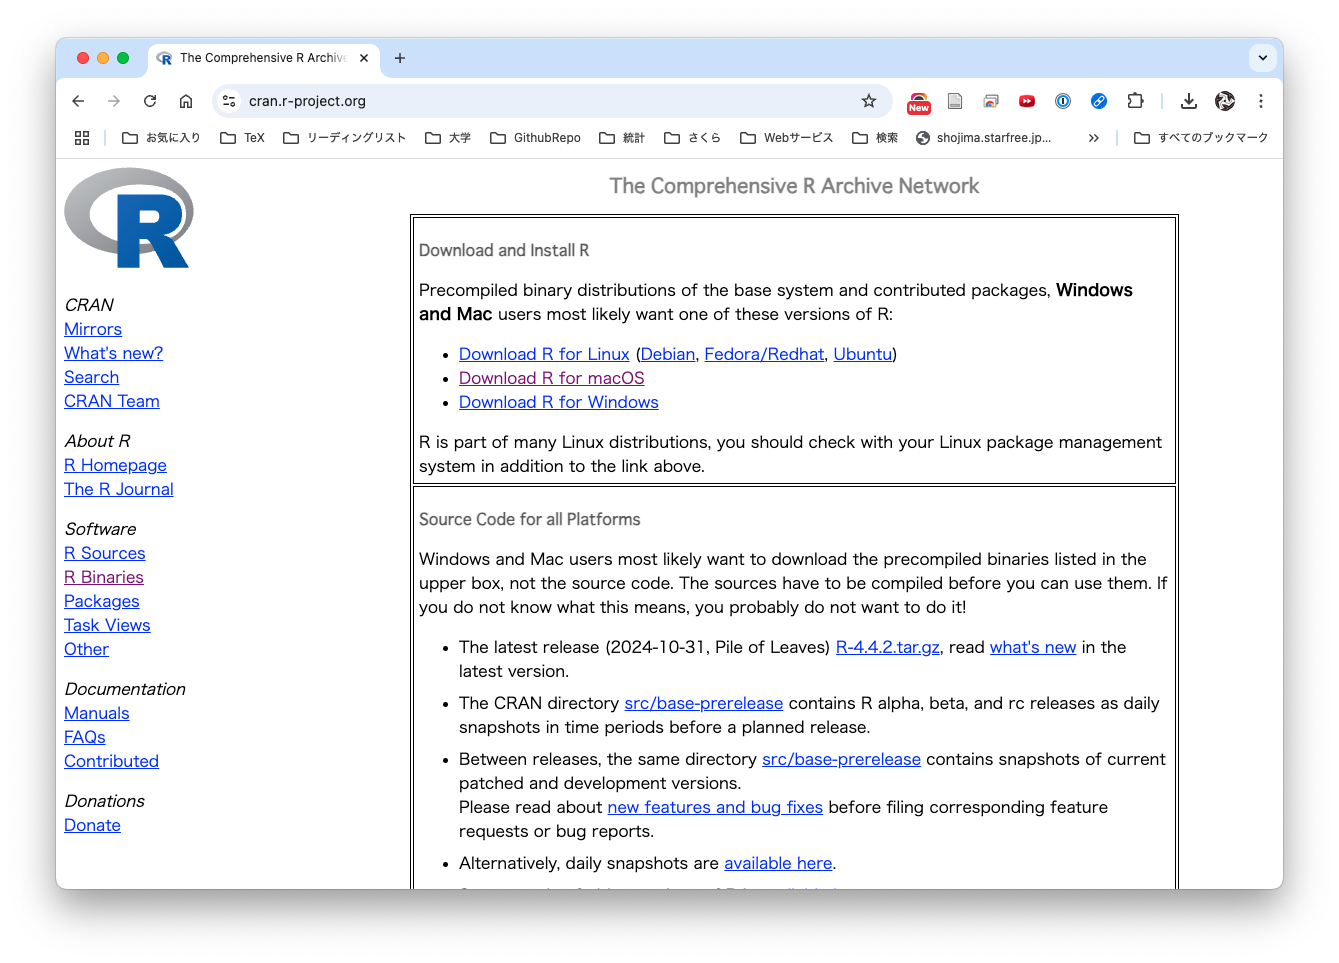
\includegraphics[keepaspectratio]{cran.png}}

}

\caption{cranのページ}

\end{figure}%

\subsection{RStudioも使いましょう}\label{rstudioux3082ux4f7fux3044ux307eux3057ux3087ux3046}

\begin{enumerate}
\def\labelenumi{\arabic{enumi}.}
\tightlist
\item
  \texttt{RStudio}で検索します。\texttt{RStudio\ Desktop}あるいはPosit社が出てきます。
\item
  \texttt{Install\ RStudio}からRStudio
  Desktopをダウンロードしてインストールしましょう。
\end{enumerate}

RStudioはServer版もあります。サーバを用意すればブラウザ経由で簡単に使える利点があります。

\pandocbounded{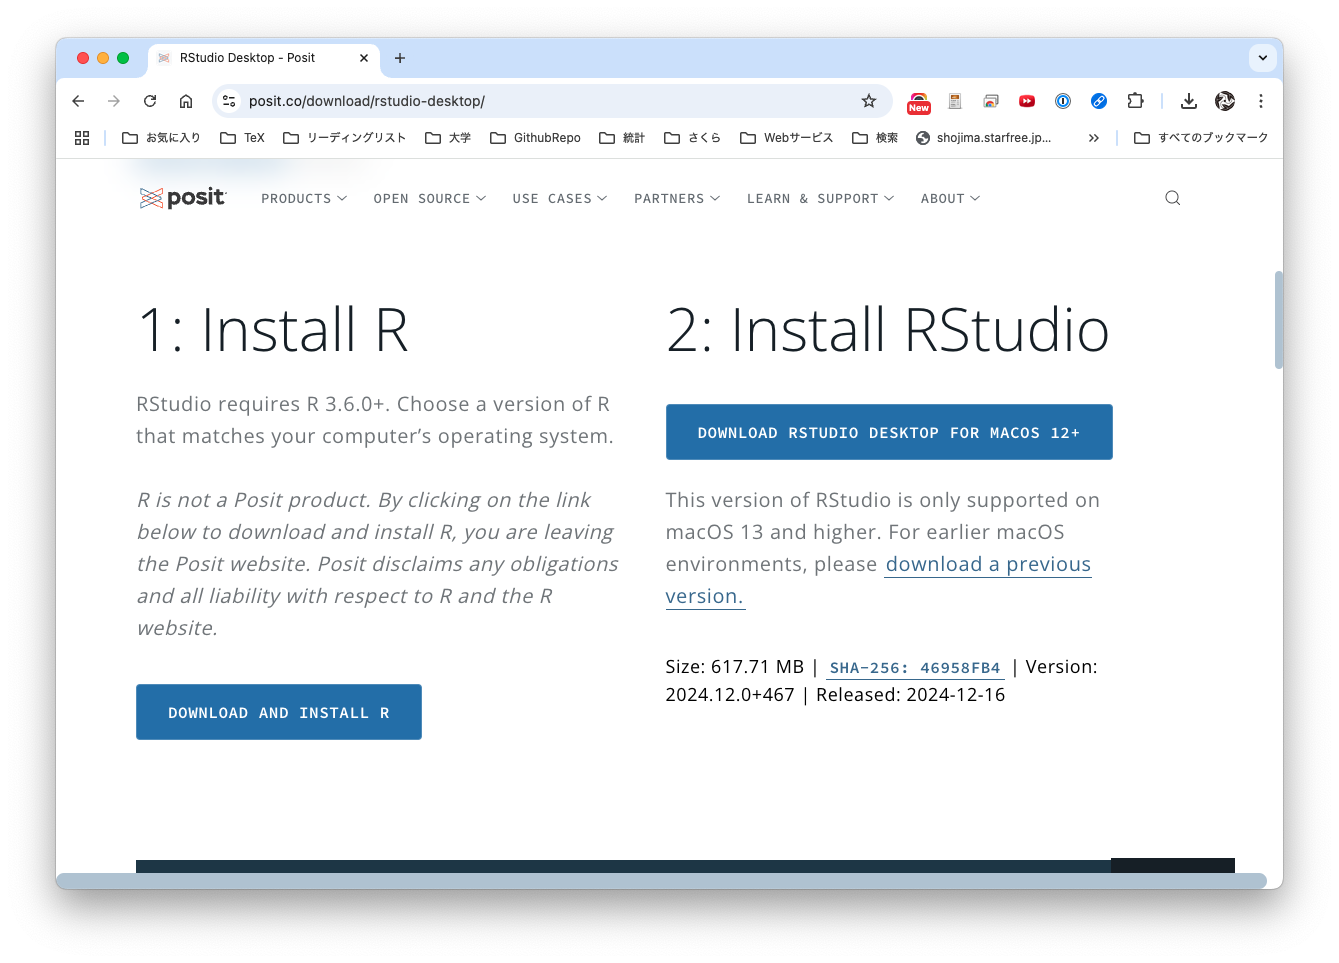
\includegraphics[keepaspectratio]{RStudio.png}}

\subsection{RStudioの起動画面}\label{rstudioux306eux8d77ux52d5ux753bux9762}

\begin{figure}[H]

{\centering \pandocbounded{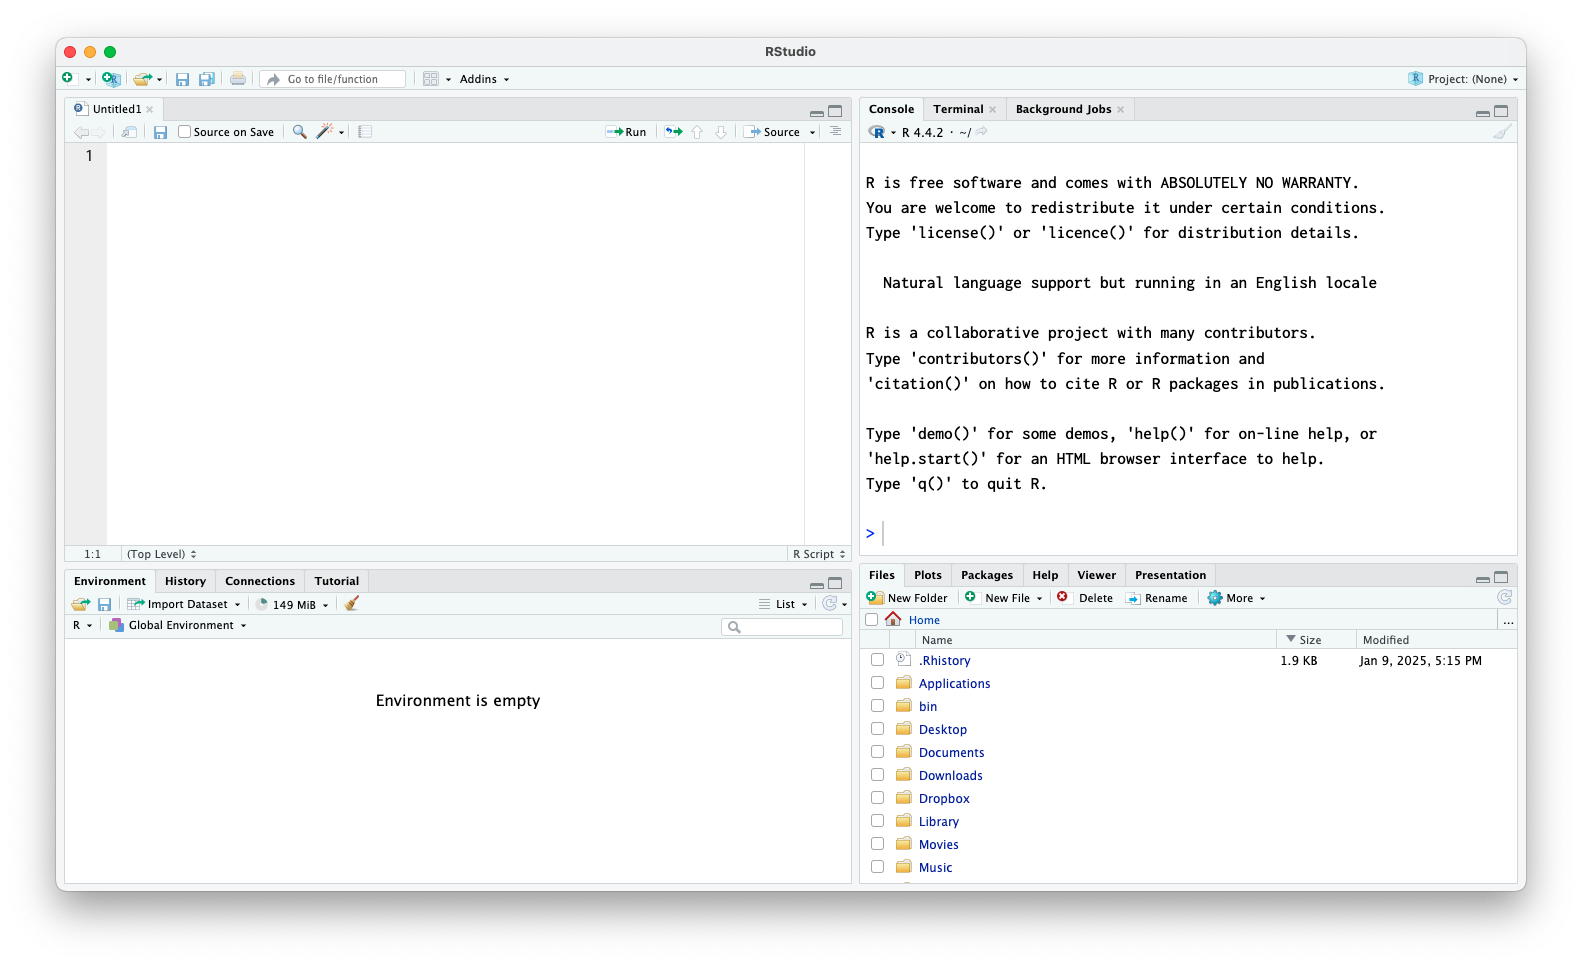
\includegraphics[keepaspectratio]{RStudioStartup.png}}

}

\caption{RStudi起動画面}

\end{figure}%

\begin{itemize}
\tightlist
\item
  大きく4分割して使います。
\item
  起動して最初にやるのが「\textbf{環境設定}」です。
\item
  メニューバーから,Tools \textgreater{} Global Optionsと進みます。
\end{itemize}

\subsection{オススメ設定}\label{ux30aaux30b9ux30b9ux30e1ux8a2dux5b9a}

\begin{figure}[H]

{\centering \pandocbounded{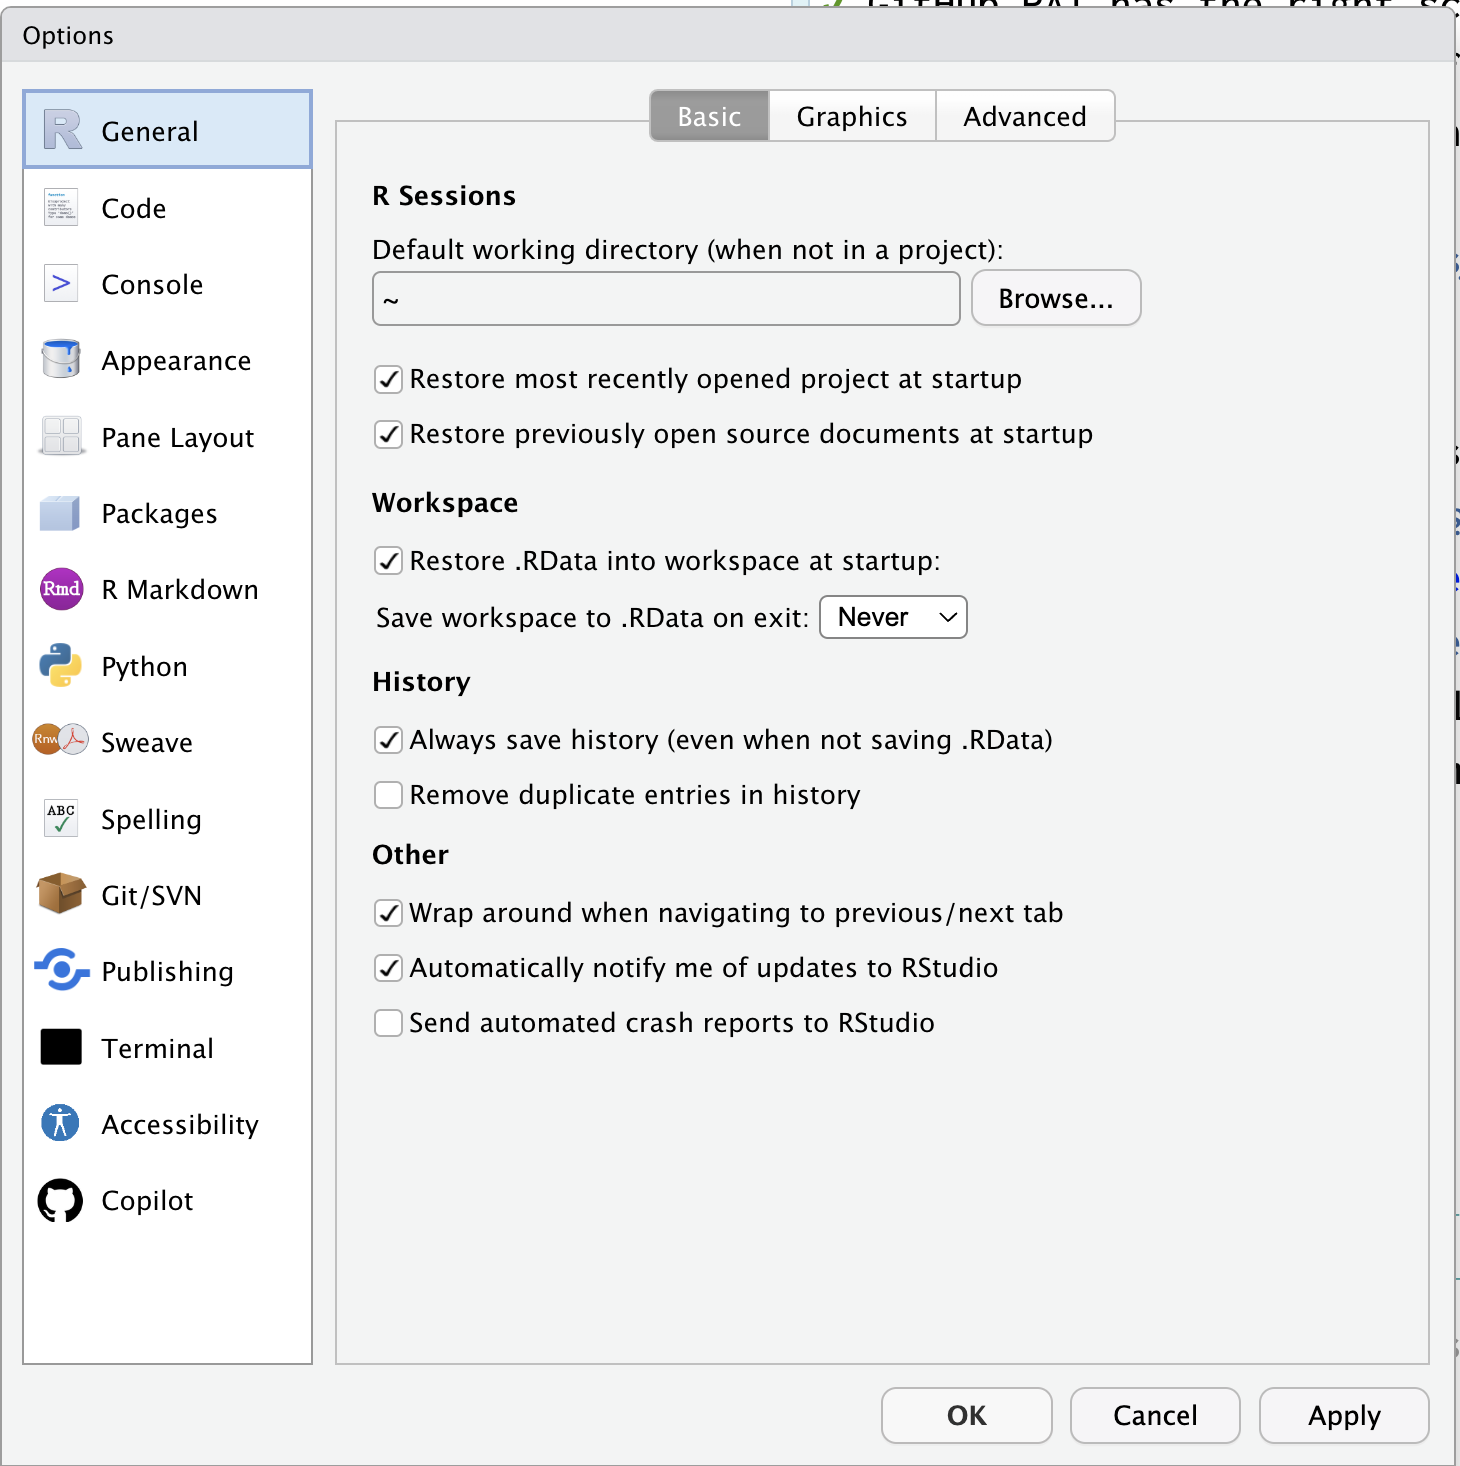
\includegraphics[keepaspectratio]{RStudioGlobalOptions.png}}

}

\caption{環境設定画面}

\end{figure}%

\begin{itemize}
\tightlist
\item
  General \textgreater{} Basic
  のWrokspace,\texttt{Save\ Workspace\ to\ .RData\ on\ exit:}を\textbf{never}に
\item
  General \textgreater{} Graphics \textgreater{} Graphics
  Deviceの\texttt{Backend}を\textbf{AGG}に
\item
  Appearance の \texttt{Editor\ Font}を見やすいフォントにしましょう
\item
  Appearance の \texttt{Editor\ Font\ size}を見やすい大きさにしましょう
\end{itemize}

おすすめフォント

\begin{itemize}
\tightlist
\item
  \href{https://github.com/yuru7/bizin-gothic}{Bizin Gothic}
\item
  \href{https://github.com/yuru7/HackGen}{HackGen}
\end{itemize}

\subsection{オススメ設定(つづき)}\label{ux30aaux30b9ux30b9ux30e1ux8a2dux5b9aux3064ux3065ux304d}

\begin{figure}[H]

{\centering \pandocbounded{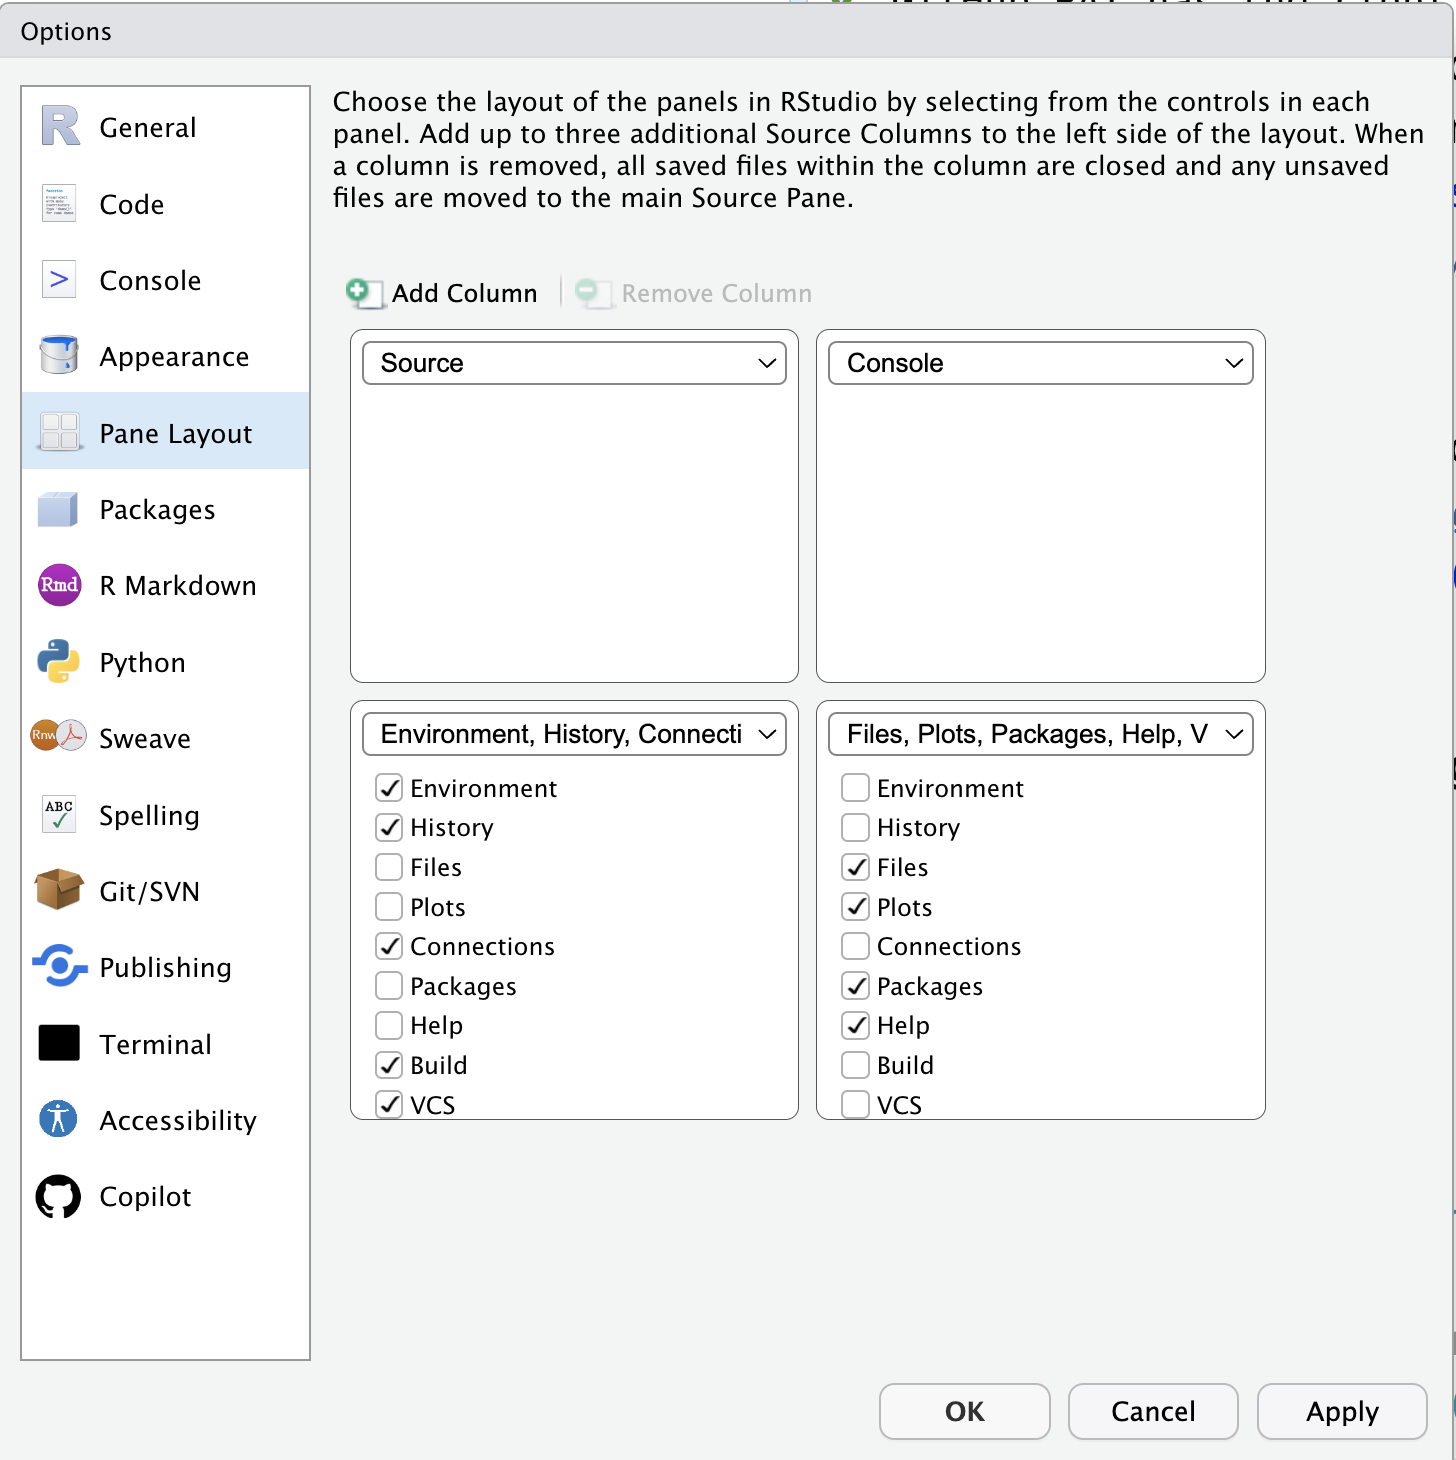
\includegraphics[keepaspectratio]{RStudioPaneLayout.png}}

}

\caption{環境設定画面その2}

\end{figure}%

\begin{itemize}
\tightlist
\item
  Pane Layoutを

  \begin{itemize}
  \tightlist
  \item
    \textbf{Source}と\textbf{Cosole}を横並びに
  \item
    かなりワイドな画面をお使いの方は,\texttt{Add\ Column}で3列にしてsource
    paneを一列増やそう
  \end{itemize}
\item
  設定が終わったら \textbf{Apply(適用)} ボタンをおして,\textbf{OK}
  で閉じる
\end{itemize}

\subsection{RStudioの4つの窓}\label{rstudioux306e4ux3064ux306eux7a93}

\begin{figure}[H]

{\centering \pandocbounded{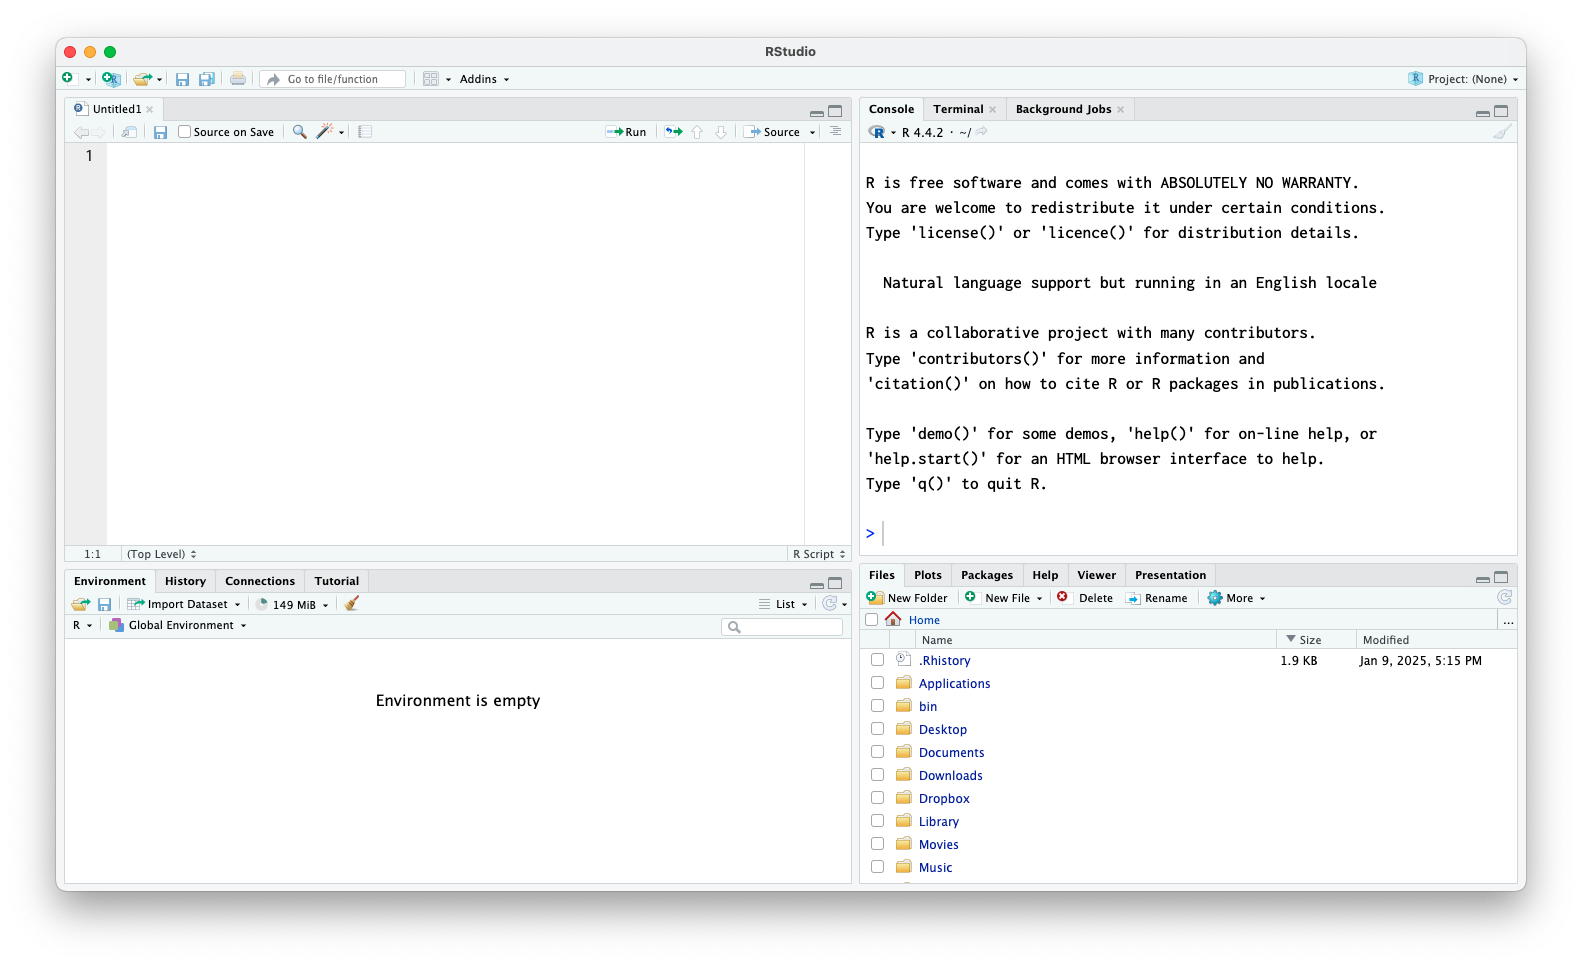
\includegraphics[keepaspectratio]{RStudioStartup.png}}

}

\caption{4つのペイン}

\end{figure}%

\begin{itemize}
\tightlist
\item
  \texttt{Source}ペインはエディタ領域で,Rスクリプトを書く場所。
\item
  \texttt{Console}ペインはRエンジン。直接Rコードを書いてもいいし,\texttt{Source}から一行ずつ,あるいは\texttt{Source}全体を流し込んで計算を実行する。
\end{itemize}

\subsection{RStudioの4つの窓}\label{rstudioux306e4ux3064ux306eux7a93-1}

\begin{figure}[H]

{\centering \pandocbounded{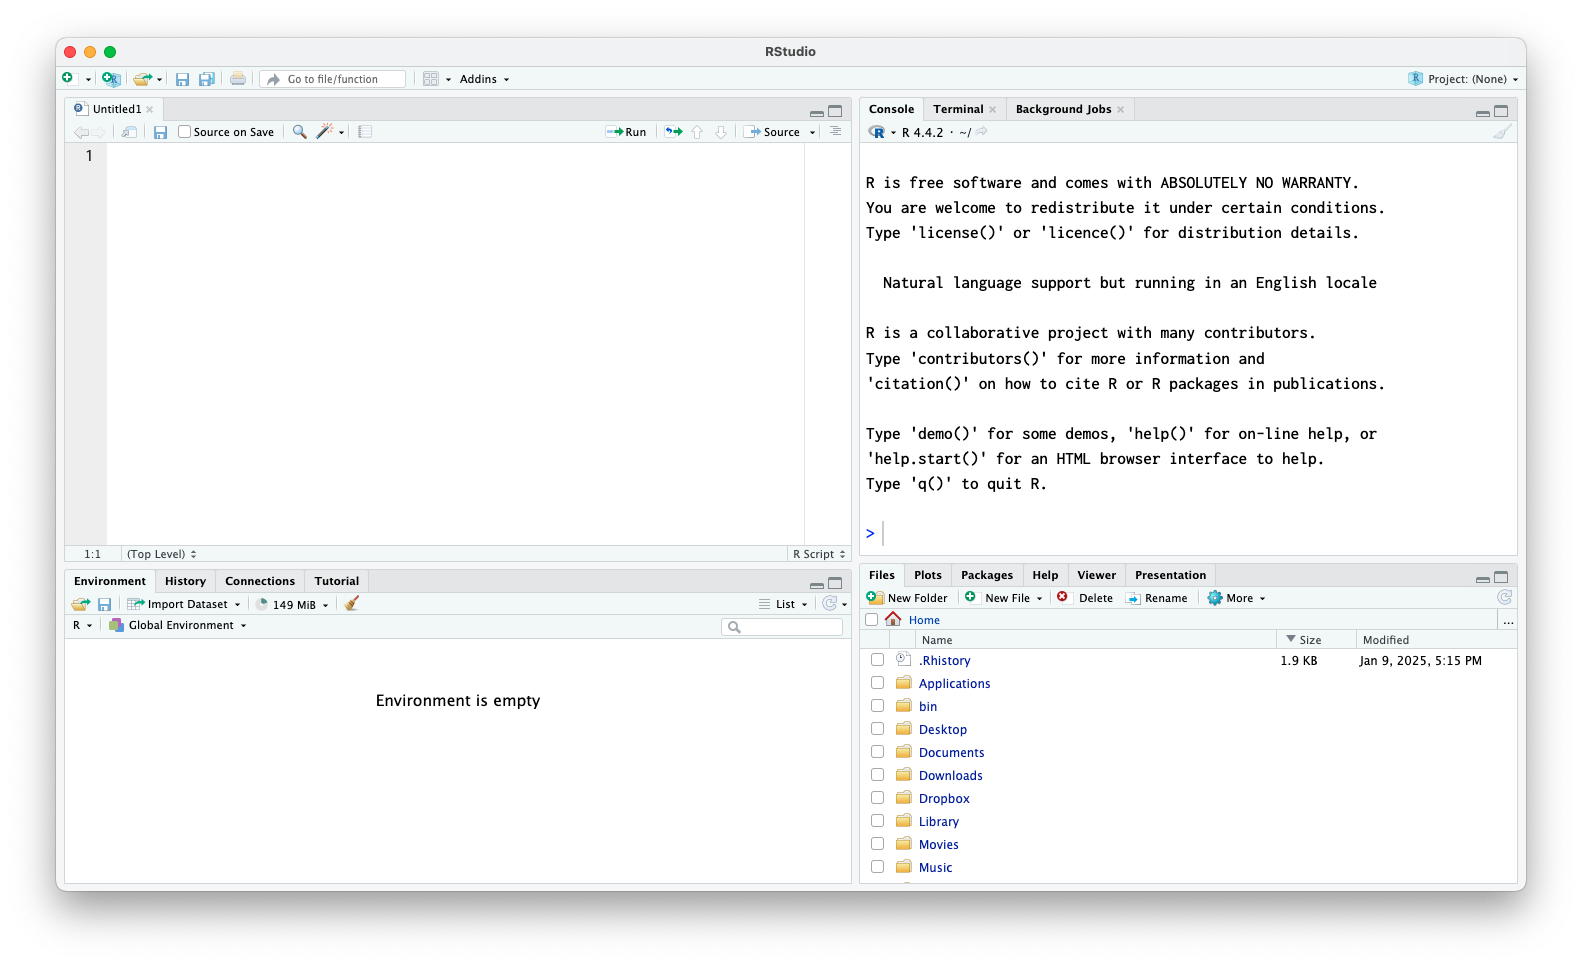
\includegraphics[keepaspectratio]{RStudioStartup.png}}

}

\caption{ペインの確認1}

\end{figure}%

\begin{itemize}
\tightlist
\item
  \texttt{Environment}はメモリに入っている変数・オブジェクトを表示
\item
  \texttt{Files}はワーキングディレクトリの表示,簡単な操作
\item
  \texttt{Package}はパッケージ管理(後述)
\item
  \texttt{Plots},\texttt{Viewer}は出力表示
\end{itemize}

\subsection{Rはプロジェクト管理が基本}\label{rux306fux30d7ux30edux30b8ux30a7ux30afux30c8ux7ba1ux7406ux304cux57faux672c}

\begin{itemize}
\tightlist
\item
  プロジェクト=フォルダに紐づいた作業環境を作ろう

  \begin{itemize}
  \tightlist
  \item
    File \textgreater{} New ProjectからNew Directory/Existing
    Directory/Version Controlを選ぶ

    \begin{itemize}
    \tightlist
    \item
      New Directory; 新しいフォルダで作業開始
    \item
      Existing Directory; 既存のフォルダをプロジェクトと紐付け
    \item
      Version Control; Githubレポジトリとプロジェクトを紐付け
    \end{itemize}
  \end{itemize}
\end{itemize}

プロジェクトにしておくと,作業フォルダの設定も自動でなされるから,ファイルの読み込みなどでパスの指定が楽になります。

\begin{itemize}
\tightlist
\item
  今回の春セミ用にプロジェクトフォルダを作りましょう!

  \begin{itemize}
  \tightlist
  \item
    すでにフォルダに色々まとめている人は,Existing Directoryから
  \item
    まだフォルダがない人は,New Directoryから
  \end{itemize}
\end{itemize}

\section{Rをさわってみましょう}\label{rux3092ux3055ux308fux3063ux3066ux307fux307eux3057ux3087ux3046}

\subsection{はじめの1歩}\label{ux306fux3058ux3081ux306e1ux6b69}

\begin{itemize}
\tightlist
\item
  Rはインタプリタ言語=一問一答

  \begin{itemize}
  \tightlist
  \item
    Consoleに\texttt{\textgreater{}}が出ていたら聞く準備ができています。
  \item
    Consoleに\texttt{+}が出ていたら前の入力が終わってません。
  \end{itemize}
\item
  直接Consoleに書き込むのではなく,スクリプトに書きましょう。

  \begin{itemize}
  \tightlist
  \item
    File \textgreater{} New File \textgreater{} R Script
    と進むと無名のスクリプトファイルが開きます
  \end{itemize}
\item
  スクリプトファイルが開いたら,まず次のように書きます。
\end{itemize}

\begin{Shaded}
\begin{Highlighting}[]
\FunctionTok{rm}\NormalTok{(}\AttributeTok{list =} \FunctionTok{ls}\NormalTok{())}
\end{Highlighting}
\end{Shaded}

\begin{itemize}
\tightlist
\item
  一行目は呪文のようなものだと思ってください。

  \begin{itemize}
  \tightlist
  \item
    \texttt{rm}という関数はremoveを意味していて,現在Rのメモリにある変数やオブジェクトを除外します。
  \item
    \texttt{list=ls()}は「メモリのすべてのオブジェクトリスト」を意味するので,これで環境の初期化になります。
  \end{itemize}
\end{itemize}

\subsection{パッケージ}\label{ux30d1ux30c3ux30b1ux30fcux30b8}

\begin{itemize}
\tightlist
\item
  パッケージは関数のセット。元のRに追加するだけで機能が増えます。
\item
  パッケージはCRANを通じて公開され,ペインの\texttt{Packages}タブで管理できます。
\end{itemize}

\pandocbounded{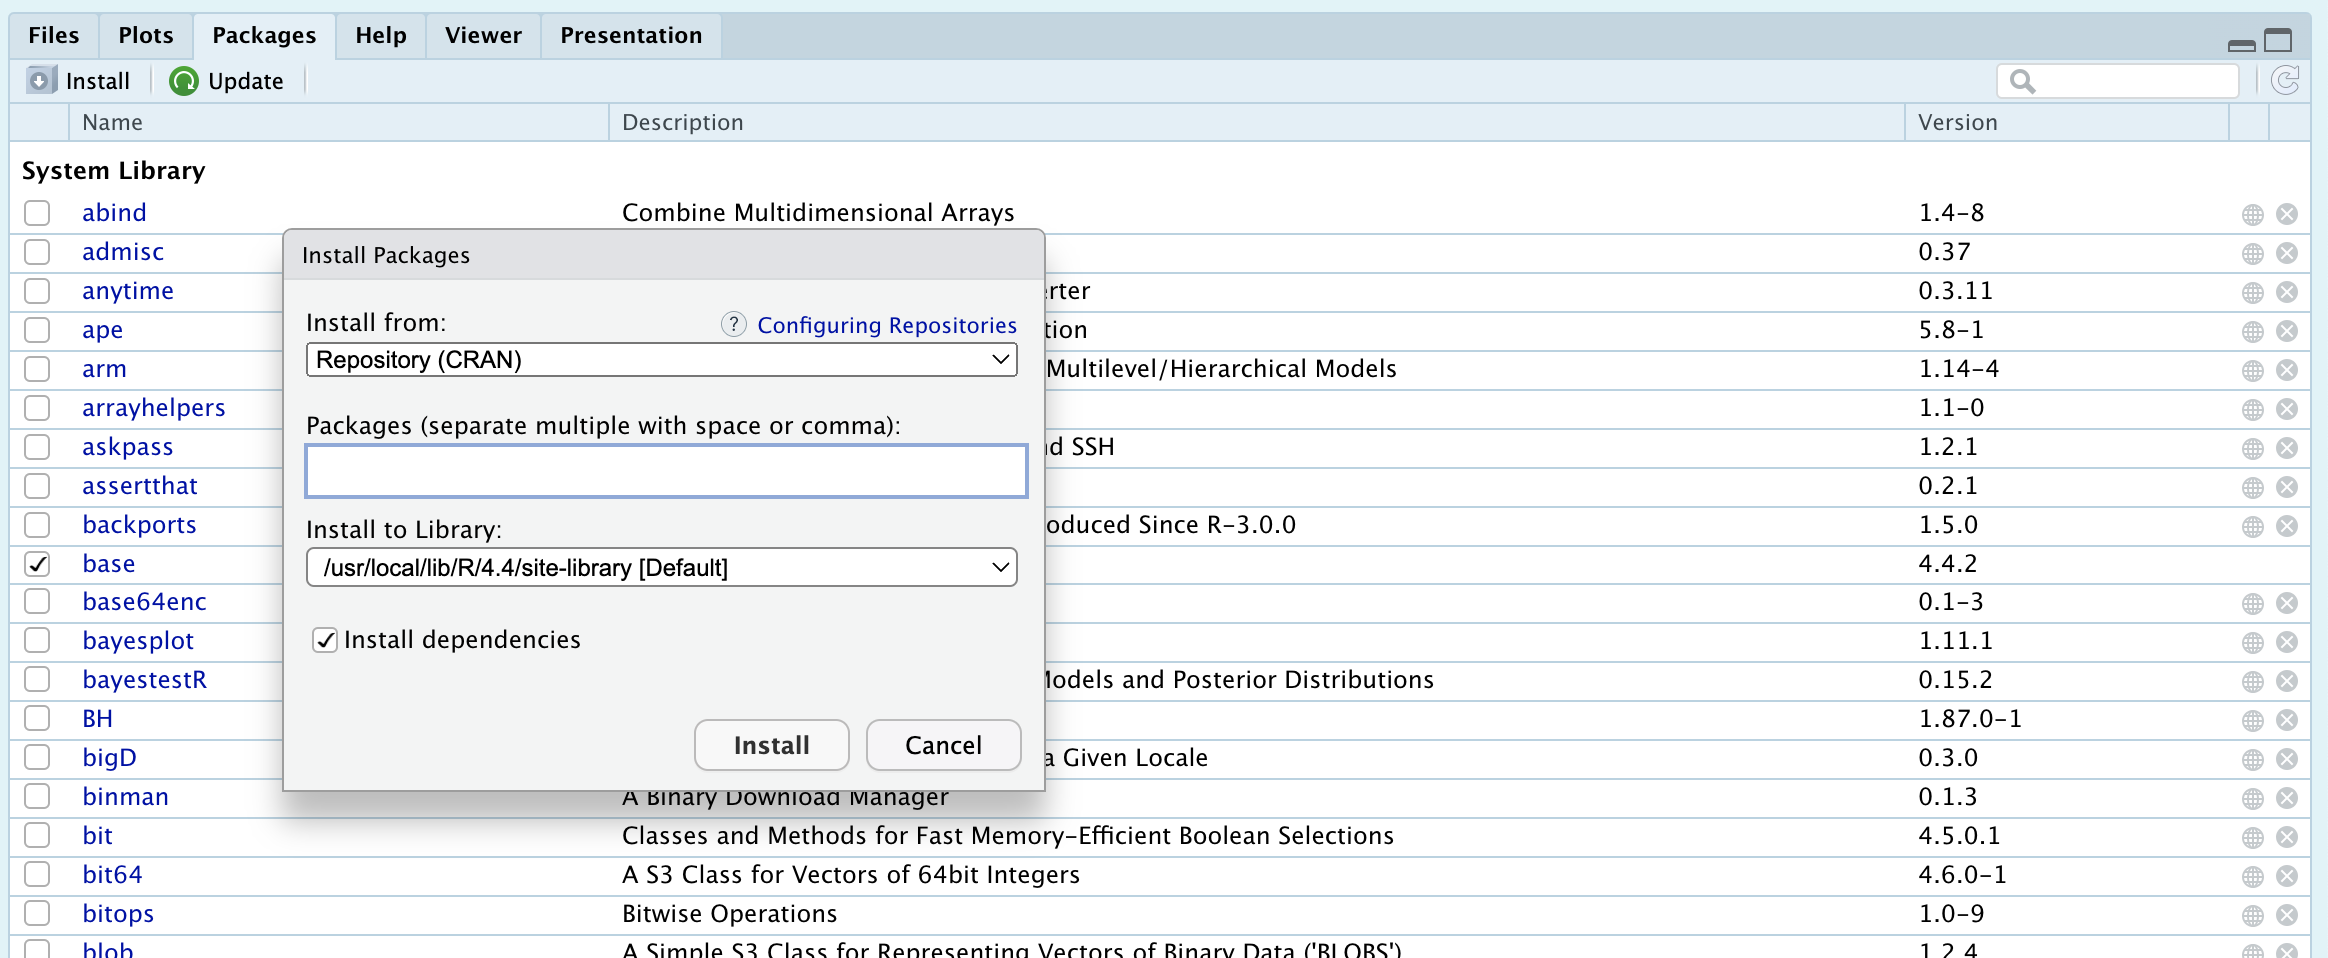
\includegraphics[keepaspectratio]{packages_tab.png}}

\begin{itemize}
\tightlist
\item
  デフォルトではCRANから取ってくることになります。(要ネット環境)

  \begin{itemize}
  \tightlist
  \item
    Packagesのところで\texttt{exametrika}と入力してインストールしちゃいましょう。
  \item
    あるパッケージが他のパッケージを必要とすることもあります。これを\textbf{依存パッケージ}といいます。
  \item
    RStudioのPackagesタブでは\texttt{install\ dependencies}にチェックがあるのがデフォルトです。

    \begin{itemize}
    \tightlist
    \item
      依存パッケージがあれば自動的にインストールされます。
    \item
      \texttt{exametrika}は\texttt{igraph}などに依存していますので,それらが同時に導入されます
    \end{itemize}
  \end{itemize}
\end{itemize}

\subsection{パッケージの使い方}\label{ux30d1ux30c3ux30b1ux30fcux30b8ux306eux4f7fux3044ux65b9}

\begin{itemize}
\tightlist
\item
  パッケージを使うには\texttt{library}と書きます。
\end{itemize}

\begin{Shaded}
\begin{Highlighting}[]
\FunctionTok{library}\NormalTok{(exametrika)}
\end{Highlighting}
\end{Shaded}

\begin{verbatim}
Loading required package: mvtnorm
\end{verbatim}

\begin{verbatim}
Loading required package: igraph
\end{verbatim}

\begin{verbatim}

Attaching package: 'igraph'
\end{verbatim}

\begin{verbatim}
The following objects are masked from 'package:stats':

    decompose, spectrum
\end{verbatim}

\begin{verbatim}
The following object is masked from 'package:base':

    union
\end{verbatim}

\begin{itemize}
\item
  これで\texttt{exametrika}パッケージの持つ関数が実行できるようになりました!他のパッケージも同様です。
\item
  パッケージのインストールを毎回する必要はありません。インストールは「手に入れる」ということだからです。
\item
  パッケージの実装(\texttt{library})はセッション毎に行う必要があります。これは「そうびする」ようなものです。
\item
  Rスクリプトの冒頭で\texttt{rm(list=ls())}としましたが,分析に必要なパッケージはスクリプトの最上部にまとめて書いておきましょう。

  \begin{itemize}
  \tightlist
  \item
    Rはインタプリタなので,逐次的に処理が進みますが,行ったり来たりしていると「パッケージを読み込んだっけ?」とか「今は何の数字で何の計算をしてるんだっけ?」となってしまいます。
  \item
    細かいことですが,パッケージは読み込む順番に影響されることがあります。

    \begin{itemize}
    \tightlist
    \item
      同じ関数名を異なるパッケージが使っている場合,後で読み込まれた方が上書きされます。
    \item
      混同しないように\texttt{PackageName::function}のように\texttt{::}で明示することがあります。
    \end{itemize}
  \end{itemize}
\end{itemize}

\subsection{数値計算の基礎}\label{ux6570ux5024ux8a08ux7b97ux306eux57faux790e}

\begin{itemize}
\tightlist
\item
  スクリプトに四則演算を書いて,Cmd+Enterでコンソールに送ります。
\item
  複数行選択/Runボタン/Sourceボタンをつかってもいいでしょう。
\end{itemize}

\begin{Shaded}
\begin{Highlighting}[]
\DecValTok{1} \SpecialCharTok{+} \DecValTok{2}
\end{Highlighting}
\end{Shaded}

\begin{verbatim}
[1] 3
\end{verbatim}

\begin{Shaded}
\begin{Highlighting}[]
\DecValTok{3} \SpecialCharTok{{-}} \DecValTok{4}
\end{Highlighting}
\end{Shaded}

\begin{verbatim}
[1] -1
\end{verbatim}

\begin{Shaded}
\begin{Highlighting}[]
\DecValTok{5} \SpecialCharTok{*} \DecValTok{6}
\end{Highlighting}
\end{Shaded}

\begin{verbatim}
[1] 30
\end{verbatim}

\begin{Shaded}
\begin{Highlighting}[]
\DecValTok{7} \SpecialCharTok{/} \DecValTok{3}
\end{Highlighting}
\end{Shaded}

\begin{verbatim}
[1] 2.333333
\end{verbatim}

\begin{itemize}
\tightlist
\item
  出力に\texttt{{[}1{]}}とあるのは気にしないでください。

  \begin{itemize}
  \tightlist
  \item
    Rはベクトルで処理します。今回の演算も,要素が1つのベクトルとして考えて処理しています。
  \end{itemize}
\end{itemize}

\subsection{数値計算の基礎}\label{ux6570ux5024ux8a08ux7b97ux306eux57faux790e-1}

\begin{itemize}
\tightlist
\item
  計算結果を保持する,あるいは名前をつけて管理することができます。
\item
  Rは「名前をつけて管理する対象」をすべて\textbf{オブジェクト}といいます。
\end{itemize}

\begin{Shaded}
\begin{Highlighting}[]
\NormalTok{a }\OtherTok{\textless{}{-}} \DecValTok{1} \SpecialCharTok{+} \DecValTok{2}
\NormalTok{b }\OtherTok{\textless{}{-}} \DecValTok{3} \SpecialCharTok{{-}} \DecValTok{4}
\FunctionTok{print}\NormalTok{(a)}
\end{Highlighting}
\end{Shaded}

\begin{verbatim}
[1] 3
\end{verbatim}

\begin{Shaded}
\begin{Highlighting}[]
\FunctionTok{print}\NormalTok{(b)}
\end{Highlighting}
\end{Shaded}

\begin{verbatim}
[1] -1
\end{verbatim}

\begin{Shaded}
\begin{Highlighting}[]
\FunctionTok{print}\NormalTok{(a }\SpecialCharTok{+}\NormalTok{ b)}
\end{Highlighting}
\end{Shaded}

\begin{verbatim}
[1] 2
\end{verbatim}

\begin{itemize}
\tightlist
\item
  \texttt{\textless{}-}で代入を意味します。ショートカット(ALTと-,optionと-)も覚えておこう
\item
  RStudioの\texttt{Environment}タブに保存されているオブジェクトが表示されています。ダブルクリックで確認できます。
\end{itemize}

\begin{Shaded}
\begin{Highlighting}[]
\NormalTok{a }\OtherTok{\textless{}{-}} \DecValTok{5}
\NormalTok{a }\SpecialCharTok{+}\NormalTok{ b}
\end{Highlighting}
\end{Shaded}

\begin{verbatim}
[1] 4
\end{verbatim}

同じオブジェクト名なら上書きされることに注意

\subsection{ベクトル,行列,リスト,データフレーム}\label{ux30d9ux30afux30c8ux30ebux884cux5217ux30eaux30b9ux30c8ux30c7ux30fcux30bfux30d5ux30ecux30fcux30e0}

\begin{itemize}
\tightlist
\item
  複数の数字のセット,\textbf{ベクトル}は\texttt{c()}でくくることで表現します。

  \begin{itemize}
  \tightlist
  \item
    連続した数字はコロン\texttt{:}で表現します。
  \end{itemize}
\item
  2次元に並ぶ数字のセット,\textbf{行列}は\texttt{matrix()}でつくります。

  \begin{itemize}
  \tightlist
  \item
    \texttt{matrix}関数にベクトルを与えるなどします。
  \end{itemize}
\item
  3次元以上の数字のセット,\textbf{配列}は\texttt{array()}で,\texttt{dim}オプションで各次元の大きさを指定します。
\item
  数字,文字,論理値(T/F)などが混在するもののセット,\textbf{リスト}は\texttt{list()}でつくります。
\item
  リストの中でも矩形に整っている\textbf{データフレーム}は,\texttt{data.frame()}でつくります。
\end{itemize}

分析するときはデータフレームがもっともよく使われます

データフレームの上位互換,\texttt{tibble}という型もあります。これは\texttt{tibble}パッケージを読み込むことで使えるようになります。

\subsection{ベクトル(Vector)の例}\label{ux30d9ux30afux30c8ux30ebvectorux306eux4f8b}

\subsubsection{数値ベクトル}\label{ux6570ux5024ux30d9ux30afux30c8ux30eb}

\begin{Shaded}
\begin{Highlighting}[]
\NormalTok{x }\OtherTok{\textless{}{-}} \FunctionTok{c}\NormalTok{(}\DecValTok{1}\NormalTok{, }\DecValTok{2}\NormalTok{, }\DecValTok{3}\NormalTok{, }\DecValTok{4}\NormalTok{, }\DecValTok{5}\NormalTok{)}
\FunctionTok{print}\NormalTok{(x)}
\end{Highlighting}
\end{Shaded}

\begin{verbatim}
[1] 1 2 3 4 5
\end{verbatim}

\subsubsection{文字列ベクトル}\label{ux6587ux5b57ux5217ux30d9ux30afux30c8ux30eb}

\begin{Shaded}
\begin{Highlighting}[]
\NormalTok{y }\OtherTok{\textless{}{-}} \FunctionTok{c}\NormalTok{(}\StringTok{"りんご"}\NormalTok{, }\StringTok{"みかん"}\NormalTok{, }\StringTok{"バナナ"}\NormalTok{)}
\FunctionTok{print}\NormalTok{(y)}
\end{Highlighting}
\end{Shaded}

\begin{verbatim}
[1] "りんご" "みかん" "バナナ"
\end{verbatim}

\subsubsection{論理値ベクトル}\label{ux8ad6ux7406ux5024ux30d9ux30afux30c8ux30eb}

\begin{itemize}
\tightlist
\item
  Rには文字,数字以外に論理値というのがあります。真/TRUEか偽/FALSEか,を表します。
\item
  使い方としては,論理判断の条件で使ったり,オプションの「スイッチオン・オフ」を表す時につかいます。
\item
  大文字の\texttt{T}や\texttt{F}は論理値を表す特別な用語(予約語)です。
\end{itemize}

\begin{Shaded}
\begin{Highlighting}[]
\NormalTok{z }\OtherTok{\textless{}{-}} \FunctionTok{c}\NormalTok{(}\ConstantTok{TRUE}\NormalTok{, }\ConstantTok{FALSE}\NormalTok{, }\ConstantTok{TRUE}\NormalTok{)}
\FunctionTok{print}\NormalTok{(z)}
\end{Highlighting}
\end{Shaded}

\begin{verbatim}
[1]  TRUE FALSE  TRUE
\end{verbatim}

\subsection{行列(Matrix)}\label{ux884cux5217matrix}

\begin{itemize}
\tightlist
\item
  1から9までの数字で3×3行列を作成
\end{itemize}

\begin{Shaded}
\begin{Highlighting}[]
\NormalTok{m1 }\OtherTok{\textless{}{-}} \FunctionTok{matrix}\NormalTok{(}\DecValTok{1}\SpecialCharTok{:}\DecValTok{9}\NormalTok{, }\AttributeTok{nrow =} \DecValTok{3}\NormalTok{, }\AttributeTok{ncol =} \DecValTok{3}\NormalTok{)}
\FunctionTok{print}\NormalTok{(m1)}
\end{Highlighting}
\end{Shaded}

\begin{verbatim}
     [,1] [,2] [,3]
[1,]    1    4    7
[2,]    2    5    8
[3,]    3    6    9
\end{verbatim}

\begin{itemize}
\tightlist
\item
  行名と列名を付ける
\end{itemize}

\begin{Shaded}
\begin{Highlighting}[]
\NormalTok{m2 }\OtherTok{\textless{}{-}} \FunctionTok{matrix}\NormalTok{(}\DecValTok{1}\SpecialCharTok{:}\DecValTok{9}\NormalTok{,}
    \AttributeTok{nrow =} \DecValTok{3}\NormalTok{, }\AttributeTok{ncol =} \DecValTok{3}\NormalTok{,}
    \AttributeTok{dimnames =} \FunctionTok{list}\NormalTok{(}
        \FunctionTok{c}\NormalTok{(}\StringTok{"A"}\NormalTok{, }\StringTok{"B"}\NormalTok{, }\StringTok{"C"}\NormalTok{),}
        \FunctionTok{c}\NormalTok{(}\StringTok{"X"}\NormalTok{, }\StringTok{"Y"}\NormalTok{, }\StringTok{"Z"}\NormalTok{)}
\NormalTok{    )}
\NormalTok{)}
\FunctionTok{print}\NormalTok{(m2)}
\end{Highlighting}
\end{Shaded}

\begin{verbatim}
  X Y Z
A 1 4 7
B 2 5 8
C 3 6 9
\end{verbatim}

\subsection{配列(Array)}\label{ux914dux5217array}

\begin{itemize}
\tightlist
\item
  2×3×2の3次元配列を作成
\end{itemize}

\begin{Shaded}
\begin{Highlighting}[]
\NormalTok{arr }\OtherTok{\textless{}{-}} \FunctionTok{array}\NormalTok{(}\DecValTok{1}\SpecialCharTok{:}\DecValTok{12}\NormalTok{, }\AttributeTok{dim =} \FunctionTok{c}\NormalTok{(}\DecValTok{2}\NormalTok{, }\DecValTok{3}\NormalTok{, }\DecValTok{2}\NormalTok{))}
\FunctionTok{print}\NormalTok{(arr)}
\end{Highlighting}
\end{Shaded}

\begin{verbatim}
, , 1

     [,1] [,2] [,3]
[1,]    1    3    5
[2,]    2    4    6

, , 2

     [,1] [,2] [,3]
[1,]    7    9   11
[2,]    8   10   12
\end{verbatim}

\subsection{リスト(List)}\label{ux30eaux30b9ux30c8list}

\begin{itemize}
\tightlist
\item
  様々な型のデータを含むリストを作成
\end{itemize}

\begin{Shaded}
\begin{Highlighting}[]
\NormalTok{my\_list }\OtherTok{\textless{}{-}} \FunctionTok{list}\NormalTok{(}
    \AttributeTok{numbers =} \FunctionTok{c}\NormalTok{(}\DecValTok{1}\NormalTok{, }\DecValTok{2}\NormalTok{, }\DecValTok{3}\NormalTok{),}
    \AttributeTok{text =} \StringTok{"Hello"}\NormalTok{,}
    \AttributeTok{logical =} \ConstantTok{TRUE}\NormalTok{,}
    \AttributeTok{matrix =} \FunctionTok{matrix}\NormalTok{(}\DecValTok{1}\SpecialCharTok{:}\DecValTok{4}\NormalTok{, }\DecValTok{2}\NormalTok{, }\DecValTok{2}\NormalTok{)}
\NormalTok{)}
\FunctionTok{print}\NormalTok{(my\_list)}
\end{Highlighting}
\end{Shaded}

\begin{verbatim}
$numbers
[1] 1 2 3

$text
[1] "Hello"

$logical
[1] TRUE

$matrix
     [,1] [,2]
[1,]    1    3
[2,]    2    4
\end{verbatim}

\subsection{リスト(List)}\label{ux30eaux30b9ux30c8list-1}

\begin{itemize}
\tightlist
\item
  リストの要素へのアクセス

  \begin{itemize}
  \tightlist
  \item
    名前付きリストなら\texttt{\$}マークで呼び出せます
  \end{itemize}
\end{itemize}

\begin{Shaded}
\begin{Highlighting}[]
\NormalTok{my\_list}\SpecialCharTok{$}\NormalTok{numbers}
\end{Highlighting}
\end{Shaded}

\begin{verbatim}
[1] 1 2 3
\end{verbatim}

\begin{Shaded}
\begin{Highlighting}[]
\NormalTok{my\_list}\SpecialCharTok{$}\NormalTok{numbers[}\DecValTok{3}\NormalTok{]}
\end{Highlighting}
\end{Shaded}

\begin{verbatim}
[1] 3
\end{verbatim}

\begin{Shaded}
\begin{Highlighting}[]
\NormalTok{my\_list}\SpecialCharTok{$}\NormalTok{matrix[, }\DecValTok{2}\NormalTok{]}
\end{Highlighting}
\end{Shaded}

\begin{verbatim}
[1] 3 4
\end{verbatim}

\begin{Shaded}
\begin{Highlighting}[]
\NormalTok{my\_list}\SpecialCharTok{$}\NormalTok{matrix}
\end{Highlighting}
\end{Shaded}

\begin{verbatim}
     [,1] [,2]
[1,]    1    3
[2,]    2    4
\end{verbatim}

\subsection{データフレーム(Data
Frame)}\label{ux30c7ux30fcux30bfux30d5ux30ecux30fcux30e0data-frame}

\begin{itemize}
\tightlist
\item
  データフレームの作成例

  \begin{itemize}
  \tightlist
  \item
    データフレームはリストの特殊な型なので,リストを\texttt{as.data.frame}関数で変換してもOK
  \end{itemize}
\end{itemize}

\begin{Shaded}
\begin{Highlighting}[]
\NormalTok{df }\OtherTok{\textless{}{-}} \FunctionTok{data.frame}\NormalTok{(}
    \AttributeTok{name =} \FunctionTok{c}\NormalTok{(}\StringTok{"田中"}\NormalTok{, }\StringTok{"鈴木"}\NormalTok{, }\StringTok{"佐藤"}\NormalTok{),}
    \AttributeTok{age =} \FunctionTok{c}\NormalTok{(}\DecValTok{25}\NormalTok{, }\DecValTok{30}\NormalTok{, }\DecValTok{28}\NormalTok{),}
    \AttributeTok{gender =} \FunctionTok{c}\NormalTok{(}\StringTok{"M"}\NormalTok{, }\StringTok{"F"}\NormalTok{, }\StringTok{"M"}\NormalTok{),}
    \AttributeTok{height =} \FunctionTok{c}\NormalTok{(}\DecValTok{170}\NormalTok{, }\DecValTok{160}\NormalTok{, }\DecValTok{175}\NormalTok{)}
\NormalTok{)}

\FunctionTok{print}\NormalTok{(df)}
\end{Highlighting}
\end{Shaded}

\begin{verbatim}
  name age gender height
1 田中  25      M    170
2 鈴木  30      F    160
3 佐藤  28      M    175
\end{verbatim}

\begin{itemize}
\tightlist
\item
  要素へのアクセスの仕方はリストと同じです
\end{itemize}

\begin{Shaded}
\begin{Highlighting}[]
\NormalTok{df}\SpecialCharTok{$}\NormalTok{age}
\end{Highlighting}
\end{Shaded}

\begin{verbatim}
[1] 25 30 28
\end{verbatim}

\subsection{データ構造の比較}\label{ux30c7ux30fcux30bfux69cbux9020ux306eux6bd4ux8f03}

\begin{longtable}[]{@{}
  >{\raggedright\arraybackslash}p{(\linewidth - 12\tabcolsep) * \real{0.1364}}
  >{\raggedright\arraybackslash}p{(\linewidth - 12\tabcolsep) * \real{0.2273}}
  >{\raggedright\arraybackslash}p{(\linewidth - 12\tabcolsep) * \real{0.1364}}
  >{\raggedright\arraybackslash}p{(\linewidth - 12\tabcolsep) * \real{0.1364}}
  >{\raggedright\arraybackslash}p{(\linewidth - 12\tabcolsep) * \real{0.1818}}
  >{\raggedright\arraybackslash}p{(\linewidth - 12\tabcolsep) * \real{0.0909}}
  >{\raggedright\arraybackslash}p{(\linewidth - 12\tabcolsep) * \real{0.0909}}@{}}
\toprule\noalign{}
\begin{minipage}[b]{\linewidth}\raggedright
特徴
\end{minipage} & \begin{minipage}[b]{\linewidth}\raggedright
ベクトル
\end{minipage} & \begin{minipage}[b]{\linewidth}\raggedright
行列
\end{minipage} & \begin{minipage}[b]{\linewidth}\raggedright
配列
\end{minipage} & \begin{minipage}[b]{\linewidth}\raggedright
リスト
\end{minipage} & \begin{minipage}[b]{\linewidth}\raggedright
df
\end{minipage} & \begin{minipage}[b]{\linewidth}\raggedright
Tibble
\end{minipage} \\
\midrule\noalign{}
\endhead
\bottomrule\noalign{}
\endlastfoot
次元 & 1次元 & 2次元 & n次元 & 階層構造 & 2次元 & 2次元 \\
型の統一 & 必要 & 必要 & 必要 & 不要 & 列ごと & 列ごと \\
データ型 & 単一 & 単一 & 単一 & 複数可 & 複数可 & 複数可 \\
主な用途 & 単純な数列 & 数値計算 & 多次元データ & 複雑なデータ &
データ分析 & データ分析 \\
\end{longtable}

tibble型はデータフレームの上位互換で,\texttt{tibble}パッケージを使うことで導入できます。主な特徴は次のとおりです。

\begin{itemize}
\tightlist
\item
  型情報の表示
\item
  行数と列数の表示
\item
  データの一部のみ表示(大きなデータセット時に便利)
\end{itemize}

\subsection{パイプ演算子を活用しよう}\label{ux30d1ux30a4ux30d7ux6f14ux7b97ux5b50ux3092ux6d3bux7528ux3057ux3088ux3046}

\begin{itemize}
\tightlist
\item
  パイプ演算子は、データの処理を順番に繋げてくれる記号
\item
  左から右へ、データが流れていくイメージ!コードが読みやすく、理解しやすくなる
\end{itemize}

\subsubsection{基本的な使い方}\label{ux57faux672cux7684ux306aux4f7fux3044ux65b9}

\begin{itemize}
\tightlist
\item
  パイプ演算子を使わないでいると?
\end{itemize}

\begin{Shaded}
\begin{Highlighting}[]
\NormalTok{result }\OtherTok{\textless{}{-}} \FunctionTok{sum}\NormalTok{(}\FunctionTok{sqrt}\NormalTok{(}\FunctionTok{abs}\NormalTok{(}\FunctionTok{log}\NormalTok{(}\FunctionTok{c}\NormalTok{(}\DecValTok{1}\SpecialCharTok{:}\DecValTok{10}\NormalTok{)))))}
\end{Highlighting}
\end{Shaded}

\begin{itemize}
\tightlist
\item
  パイプ演算子を使ってみると?
\end{itemize}

\begin{Shaded}
\begin{Highlighting}[]
\NormalTok{result }\OtherTok{\textless{}{-}} \FunctionTok{c}\NormalTok{(}\DecValTok{1}\SpecialCharTok{:}\DecValTok{10}\NormalTok{) }\SpecialCharTok{|\textgreater{}}
    \FunctionTok{log}\NormalTok{() }\SpecialCharTok{|\textgreater{}}
    \FunctionTok{abs}\NormalTok{() }\SpecialCharTok{|\textgreater{}}
    \FunctionTok{sqrt}\NormalTok{() }\SpecialCharTok{|\textgreater{}}
    \FunctionTok{sum}\NormalTok{()}
\end{Highlighting}
\end{Shaded}

\begin{itemize}
\tightlist
\item
  パイプ演算子はショートカット\texttt{Ctrl/Cmd\ +\ Shift\ +\ M}で入力できます

  \begin{itemize}
  \tightlist
  \item
    \texttt{\textbar{}\textgreater{}}はR4.1以降使えるようになった,Rのもってるパイプ演算子
  \item
    \texttt{\%\textgreater{}\%}は\texttt{magrittr}パッケージや,それを含んだ\texttt{tidyverse}パッケージで以前から使われていたもの
  \end{itemize}
\end{itemize}

\subsection{(余談)tidyな世界}\label{ux4f59ux8ac7tidyux306aux4e16ux754c}

\begin{itemize}
\tightlist
\item
  \texttt{tidyverse}パッケージは,データハンドリングを画期的に簡単にしたパッケージで,これでRのユーザが一気に広がったと言っても過言ではありません。
\item
  \texttt{tidyverse}パッケージはパッケージのパッケージ。

  \begin{itemize}
  \tightlist
  \item
    大規模データ用のデータフレーム,\texttt{tibble}
  \item
    パイプ演算子のパッケージ\texttt{magrittr}
  \item
    描画を綺麗にしてくれるパッケージ\texttt{ggplot2}などが含まれます
  \end{itemize}
\item
  専門の書籍も出ています
  \texttt{tidyverse}パッケージを基本にした\href{https://amzn.to/4bisTkc}{改訂2版RユーザのためのRStudio{[}実践{]}入門〜tidyverseによるモダンな分析フローの世界}
\end{itemize}

\subsection{(余談)チートシートを活用しよう}\label{ux4f59ux8ac7ux30c1ux30fcux30c8ux30b7ux30fcux30c8ux3092ux6d3bux7528ux3057ux3088ux3046}

\begin{itemize}
\tightlist
\item
  RStudioのメニューバー,Help\textgreater{} Cheat Sheetsと進んでください
\item
  PDFファイル1,2枚分で基本的な使い方を始めとした,様々なチートシートが現れます!
\end{itemize}

\pandocbounded{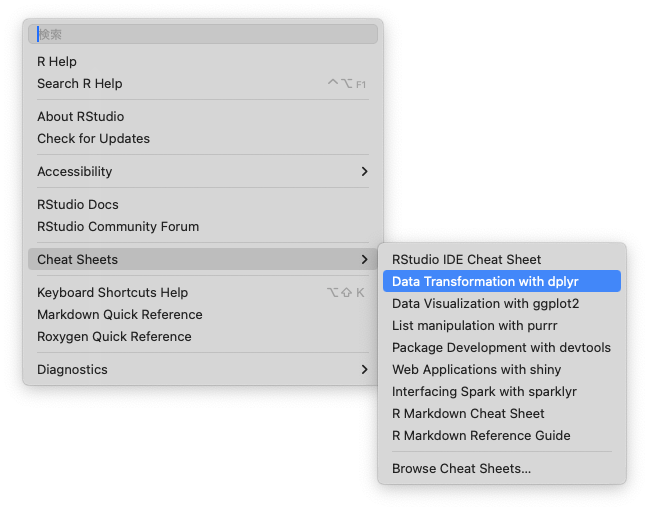
\includegraphics[keepaspectratio]{cheetSheet.png}}

\section{具体的にデータを扱ってみよう}\label{ux5177ux4f53ux7684ux306bux30c7ux30fcux30bfux3092ux6271ux3063ux3066ux307fux3088ux3046}

\subsection{データの読み込みと操作}\label{ux30c7ux30fcux30bfux306eux8aadux307fux8fbcux307fux3068ux64cdux4f5c}

\subsubsection{CSVファイルの読み込み}\label{csvux30d5ux30a1ux30a4ux30ebux306eux8aadux307fux8fbcux307f}

\begin{itemize}
\tightlist
\item
  CSVファイルはRでもっとも一般的なデータ形式の一つです
\item
  エクセルファイルなどと違って,アプリケーションに依存せず,メモ帳で開くこともできますので,あらゆるOSに対応できます。
\item
  基本的な読み込み方法は \texttt{read.csv()} 関数を使います
\item
  \texttt{tidyverse}パッケージを使っている人は,\texttt{read\_csv()}関数のほうが細かな調整が効いていいかも
\end{itemize}

\subsection{基本的なCSV読み込み}\label{ux57faux672cux7684ux306acsvux8aadux307fux8fbcux307f}

\begin{Shaded}
\begin{Highlighting}[]
\NormalTok{data }\OtherTok{\textless{}{-}} \FunctionTok{read.csv}\NormalTok{(}\StringTok{"data.csv"}\NormalTok{)}
\end{Highlighting}
\end{Shaded}

\subsubsection{日本語を含むCSVファイルの場合}\label{ux65e5ux672cux8a9eux3092ux542bux3080csvux30d5ux30a1ux30a4ux30ebux306eux5834ux5408}

\begin{itemize}
\tightlist
\item
  Windowsユーザ/Excelユーザは文字化けを起こす可能性があります。
\item
  世界標準である\texttt{UTF-8}という文字コードでファイルを管理しましょう
\end{itemize}

\begin{Shaded}
\begin{Highlighting}[]
\NormalTok{data }\OtherTok{\textless{}{-}} \FunctionTok{read.csv}\NormalTok{(}\StringTok{"data.csv"}\NormalTok{, }\AttributeTok{fileEncoding =} \StringTok{"UTF{-}8"}\NormalTok{)}
\end{Highlighting}
\end{Shaded}

\begin{itemize}
\tightlist
\item
  Rstudioの\texttt{Files}
  タブからファイルを選んで\texttt{Import\ Dataset}とするとGUIでも操作できます。

  \begin{itemize}
  \tightlist
  \item
    Excelファイルを読み込みたい場合は,そちらを使うのもいいでしょう
  \end{itemize}
\end{itemize}

\pandocbounded{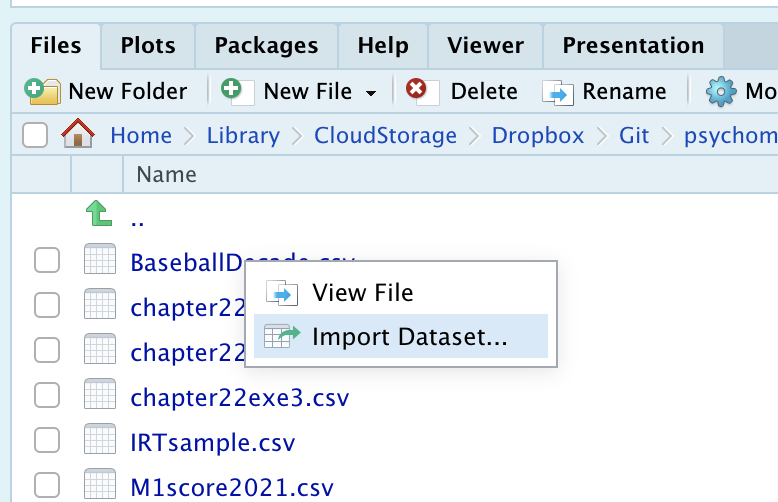
\includegraphics[keepaspectratio]{importDataset.png}}

\subsection{Import Dataset}\label{import-dataset}

\pandocbounded{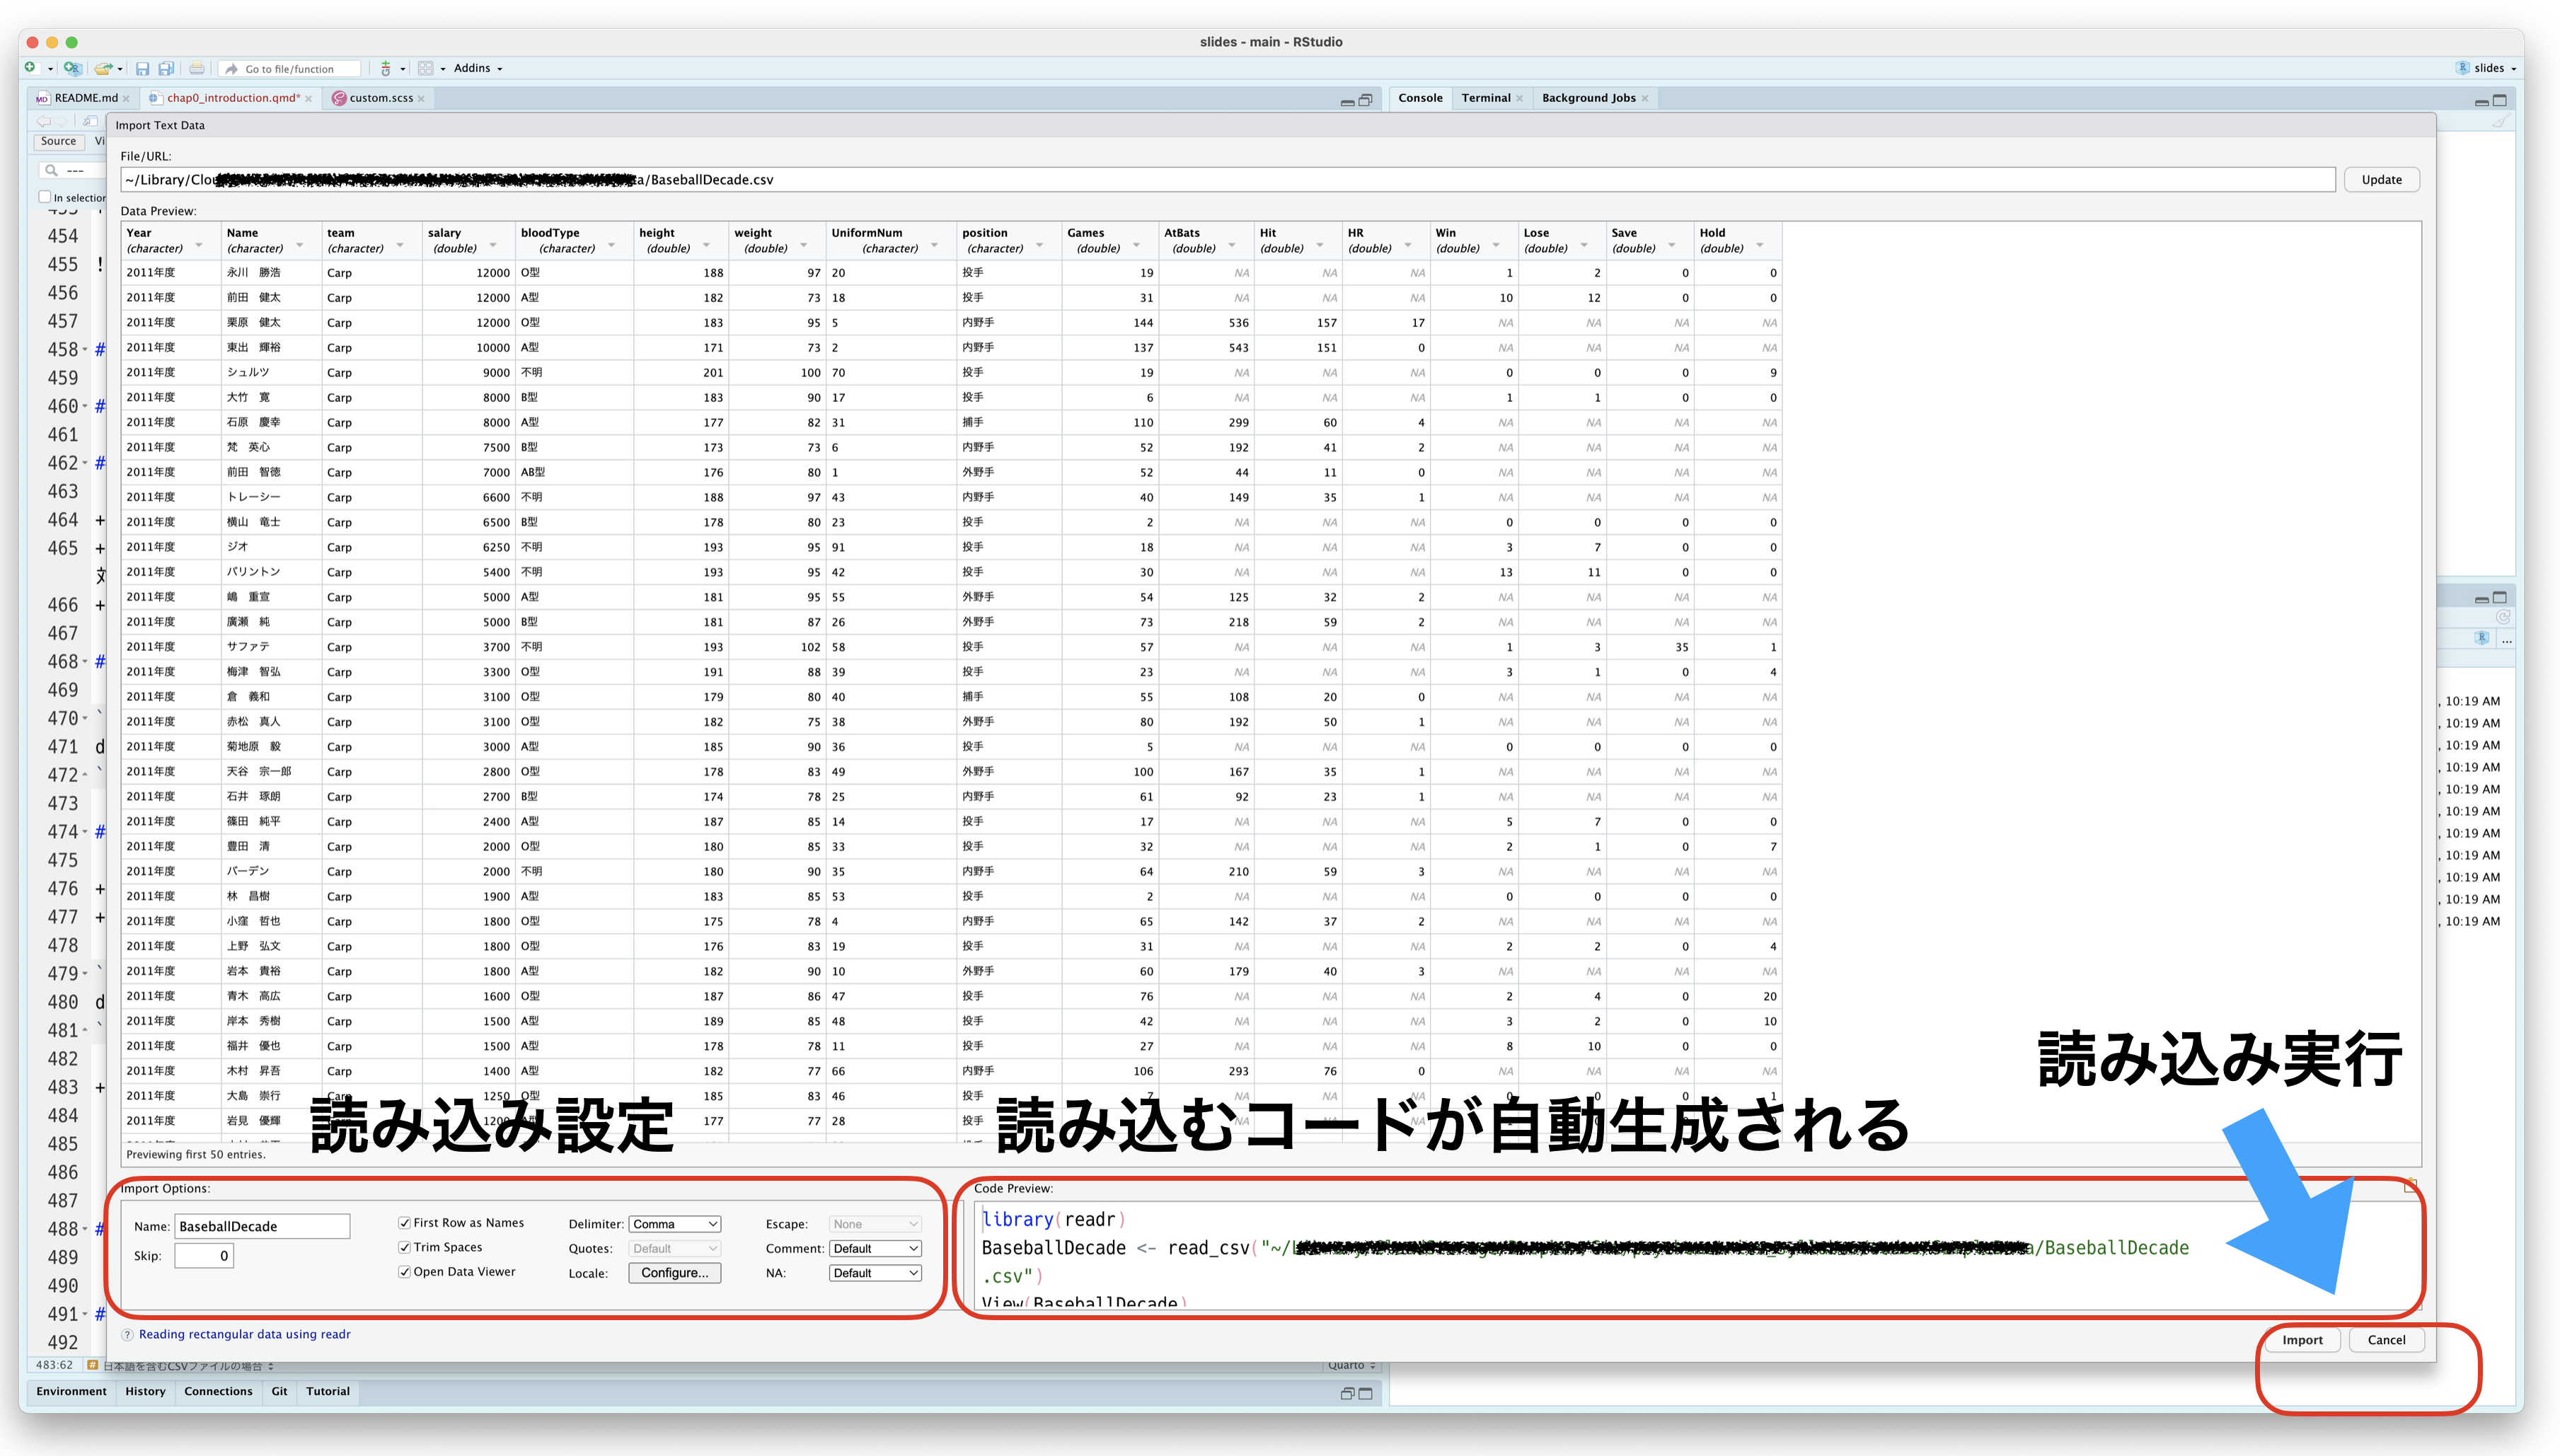
\includegraphics[keepaspectratio]{importDatasetWindow.png}}

\subsection{サンプルコードを読み込んでみよう}\label{ux30b5ux30f3ux30d7ux30ebux30b3ux30fcux30c9ux3092ux8aadux307fux8fbcux3093ux3067ux307fux3088ux3046}

\begin{itemize}
\tightlist
\item
  インターネットから読み込むこともできます!
\item
  次のコードでサンプルデータを読み込んでみましょう。
\end{itemize}

\begin{Shaded}
\begin{Highlighting}[]
\NormalTok{baseball }\OtherTok{\textless{}{-}} \FunctionTok{read.csv}\NormalTok{(}\StringTok{"https://shorturl.at/X4ctc"}\NormalTok{)}
\end{Highlighting}
\end{Shaded}

\begin{itemize}
\tightlist
\item
  ショートURLの参照先は怪しいところではありません。

  \begin{itemize}
  \tightlist
  \item
    https://kosugitti.github.io/psychometrics\_syllabus/codes/SampleData/BaseballDecade.csv
  \item
    私の\href{https://kosugitti.github.io/psychometrics_syllabus/}{心理統計教育教材}サイトに置いてあるサンプルデータです
  \item
    野球選手の基本情報など,10年分のデータがあります。
  \end{itemize}
\item
  データの一部(冒頭)を\texttt{head}関数で確認してみましょう
\end{itemize}

\begin{Shaded}
\begin{Highlighting}[]
\FunctionTok{head}\NormalTok{(baseball)}
\end{Highlighting}
\end{Shaded}

\begin{verbatim}
      Year       Name team salary bloodType height weight UniformNum position
1 2011年度 永川 勝浩 Carp  12000       O型    188     97         20     投手
2 2011年度 前田 健太 Carp  12000       A型    182     73         18     投手
3 2011年度 栗原 健太 Carp  12000       O型    183     95          5   内野手
4 2011年度 東出 輝裕 Carp  10000       A型    171     73          2   内野手
5 2011年度   シュルツ Carp   9000      不明    201    100         70     投手
6 2011年度   大竹 寛 Carp   8000       B型    183     90         17     投手
  Games AtBats Hit HR Win Lose Save Hold
1    19     NA  NA NA   1    2    0    0
2    31     NA  NA NA  10   12    0    0
3   144    536 157 17  NA   NA   NA   NA
4   137    543 151  0  NA   NA   NA   NA
5    19     NA  NA NA   0    0    0    9
6     6     NA  NA NA   1    1    0    0
\end{verbatim}

\subsection{オブジェクトの基本情報}\label{ux30aaux30d6ux30b8ux30a7ux30afux30c8ux306eux57faux672cux60c5ux5831}

\begin{itemize}
\tightlist
\item
  \texttt{str}関数,あるいは\texttt{Environment}タブにあるオブジェクト名を開くと,基本情報が確認できます。
\end{itemize}

\begin{Shaded}
\begin{Highlighting}[]
\FunctionTok{str}\NormalTok{(baseball)}
\end{Highlighting}
\end{Shaded}

\begin{verbatim}
'data.frame':   6546 obs. of  17 variables:
 $ Year      : chr  "2011年度" "2011年度" "2011年度" "2011年度" ...
 $ Name      : chr  "永川 勝浩" "前田 健太" "栗原 健太" "東出 輝裕" ...
 $ team      : chr  "Carp" "Carp" "Carp" "Carp" ...
 $ salary    : int  12000 12000 12000 10000 9000 8000 8000 7500 7000 6600 ...
 $ bloodType : chr  "O型" "A型" "O型" "A型" ...
 $ height    : int  188 182 183 171 201 183 177 173 176 188 ...
 $ weight    : int  97 73 95 73 100 90 82 73 80 97 ...
 $ UniformNum: int  20 18 5 2 70 17 31 6 1 43 ...
 $ position  : chr  "投手" "投手" "内野手" "内野手" ...
 $ Games     : int  19 31 144 137 19 6 110 52 52 40 ...
 $ AtBats    : int  NA NA 536 543 NA NA 299 192 44 149 ...
 $ Hit       : int  NA NA 157 151 NA NA 60 41 11 35 ...
 $ HR        : int  NA NA 17 0 NA NA 4 2 0 1 ...
 $ Win       : int  1 10 NA NA 0 1 NA NA NA NA ...
 $ Lose      : int  2 12 NA NA 0 1 NA NA NA NA ...
 $ Save      : int  0 0 NA NA 0 0 NA NA NA NA ...
 $ Hold      : int  0 0 NA NA 9 0 NA NA NA NA ...
\end{verbatim}

\begin{itemize}
\tightlist
\item
  何年度のデータか(\texttt{Year}),選手名(\texttt{Name}),どのチーム所属か(\texttt{team}),年俸(\texttt{salary})などがあります。
\item
  データの型もわかります

  \begin{itemize}
  \tightlist
  \item
    \texttt{chr}は文字列型です。四則演算の対象ではありません。
  \item
    \texttt{int},\texttt{num}は数字です(整数と実数)
  \item
    \texttt{NA}は欠損値を表しています。
  \end{itemize}
\item
  \texttt{read.csv}関数は読み込んだデータを自動的にデータフレーム型にします。
\end{itemize}

\subsection{記述統計量}\label{ux8a18ux8ff0ux7d71ux8a08ux91cf}

\begin{itemize}
\tightlist
\item
  \texttt{summary}関数で要約統計量を算出できます
\end{itemize}

\begin{Shaded}
\begin{Highlighting}[]
\FunctionTok{summary}\NormalTok{(baseball)}
\end{Highlighting}
\end{Shaded}

\begin{verbatim}
     Year               Name               team               salary     
 Length:6546        Length:6546        Length:6546        Min.   :  200  
 Class :character   Class :character   Class :character   1st Qu.: 1000  
 Mode  :character   Mode  :character   Mode  :character   Median : 2000  
                                                          Mean   : 5178  
                                                          3rd Qu.: 5700  
                                                          Max.   :65000  
                                                                         
  bloodType             height          weight      UniformNum   
 Length:6546        Min.   :163.0   Min.   : 60   Min.   : 0.00  
 Class :character   1st Qu.:177.0   1st Qu.: 78   1st Qu.:16.00  
 Mode  :character   Median :180.0   Median : 83   Median :33.00  
                    Mean   :180.7   Mean   : 84   Mean   :34.93  
                    3rd Qu.:184.0   3rd Qu.: 89   3rd Qu.:52.00  
                    Max.   :216.0   Max.   :135   Max.   :99.00  
                                                                 
   position             Games            AtBats           Hit        
 Length:6546        Min.   :  1.00   Min.   :  0.0   Min.   :  0.00  
 Class :character   1st Qu.:  9.00   1st Qu.: 23.0   1st Qu.:  4.00  
 Mode  :character   Median : 25.00   Median : 95.0   Median : 21.00  
                    Mean   : 40.67   Mean   :165.1   Mean   : 42.53  
                    3rd Qu.: 61.00   3rd Qu.:271.0   3rd Qu.: 69.00  
                    Max.   :144.00   Max.   :603.0   Max.   :216.00  
                                     NA's   :3233    NA's   :3233    
       HR              Win              Lose             Save      
 Min.   : 0.000   Min.   : 0.000   Min.   : 0.000   Min.   : 0.00  
 1st Qu.: 0.000   1st Qu.: 0.000   1st Qu.: 0.000   1st Qu.: 0.00  
 Median : 1.000   Median : 1.000   Median : 1.000   Median : 0.00  
 Mean   : 3.967   Mean   : 2.517   Mean   : 2.509   Mean   : 1.27  
 3rd Qu.: 4.000   3rd Qu.: 4.000   3rd Qu.: 4.000   3rd Qu.: 0.00  
 Max.   :60.000   Max.   :24.000   Max.   :15.000   Max.   :54.00  
 NA's   :3233     NA's   :3307     NA's   :3307     NA's   :3307   
      Hold       
 Min.   : 0.000  
 1st Qu.: 0.000  
 Median : 0.000  
 Mean   : 3.511  
 3rd Qu.: 3.000  
 Max.   :45.000  
 NA's   :3307    
\end{verbatim}

\begin{itemize}
\tightlist
\item
  行数,列数を確認して,データのサイズを見ておきましょう
\end{itemize}

\begin{Shaded}
\begin{Highlighting}[]
\FunctionTok{NROW}\NormalTok{(baseball)}
\end{Highlighting}
\end{Shaded}

\begin{verbatim}
[1] 6546
\end{verbatim}

\begin{Shaded}
\begin{Highlighting}[]
\FunctionTok{NCOL}\NormalTok{(baseball)}
\end{Highlighting}
\end{Shaded}

\begin{verbatim}
[1] 17
\end{verbatim}

\subsection{変数毎の要約統計量}\label{ux5909ux6570ux6bceux306eux8981ux7d04ux7d71ux8a08ux91cf}

\begin{itemize}
\tightlist
\item
  変数に\texttt{\$}でアクセスして,要約統計量を計算してみましょう。
\end{itemize}

\begin{Shaded}
\begin{Highlighting}[]
\FunctionTok{mean}\NormalTok{(baseball}\SpecialCharTok{$}\NormalTok{height)}
\end{Highlighting}
\end{Shaded}

\begin{verbatim}
[1] 180.7177
\end{verbatim}

\begin{Shaded}
\begin{Highlighting}[]
\FunctionTok{sd}\NormalTok{(baseball}\SpecialCharTok{$}\NormalTok{height)}
\end{Highlighting}
\end{Shaded}

\begin{verbatim}
[1] 5.613504
\end{verbatim}

\begin{Shaded}
\begin{Highlighting}[]
\FunctionTok{median}\NormalTok{(baseball}\SpecialCharTok{$}\NormalTok{weight)}
\end{Highlighting}
\end{Shaded}

\begin{verbatim}
[1] 83
\end{verbatim}

\begin{Shaded}
\begin{Highlighting}[]
\FunctionTok{max}\NormalTok{(baseball}\SpecialCharTok{$}\NormalTok{salary)}
\end{Highlighting}
\end{Shaded}

\begin{verbatim}
[1] 65000
\end{verbatim}

\begin{Shaded}
\begin{Highlighting}[]
\FunctionTok{min}\NormalTok{(baseball}\SpecialCharTok{$}\NormalTok{salary)}
\end{Highlighting}
\end{Shaded}

\begin{verbatim}
[1] 200
\end{verbatim}

\begin{Shaded}
\begin{Highlighting}[]
\FunctionTok{quantile}\NormalTok{(baseball}\SpecialCharTok{$}\NormalTok{salary)}
\end{Highlighting}
\end{Shaded}

\begin{verbatim}
   0%   25%   50%   75%  100% 
  200  1000  2000  5700 65000 
\end{verbatim}

\subsection{因子型をつくってみましょう}\label{ux56e0ux5b50ux578bux3092ux3064ux304fux3063ux3066ux307fux307eux3057ux3087ux3046}

\begin{itemize}
\tightlist
\item
  チーム名はたかだか12種類です。名義尺度水準+ラベルの数値であるFactor型にしてみましょう。
\end{itemize}

\begin{Shaded}
\begin{Highlighting}[]
\NormalTok{baseball}\SpecialCharTok{$}\NormalTok{team }\OtherTok{\textless{}{-}} \FunctionTok{as.factor}\NormalTok{(baseball}\SpecialCharTok{$}\NormalTok{team)}
\FunctionTok{summary}\NormalTok{(baseball}\SpecialCharTok{$}\NormalTok{team)}
\end{Highlighting}
\end{Shaded}

\begin{verbatim}
    Carp     DeNA  Dragons   Eagles Fighters   Giants    Lions    Lotte 
     517      550      573      569      533      524      528      538 
    Orix Softbank Swallows   Tigers 
     579      525      556      554 
\end{verbatim}

\begin{itemize}
\tightlist
\item
  一行目で,同じ変数に「上書き」していることに注意
\item
  \texttt{as.factor}関数は変数をFactor型に変換するものです

  \begin{itemize}
  \tightlist
  \item
    クラス名,実験の水準などグループ化変数として扱うのに便利です
  \end{itemize}
\end{itemize}

\subsection{可視化してみましょう}\label{ux53efux8996ux5316ux3057ux3066ux307fux307eux3057ux3087ux3046}

\begin{itemize}
\tightlist
\item
  \textbf{データは図にする}のが基本です。Rの基本関数でも十分綺麗な図が描けます。

  \begin{itemize}
  \tightlist
  \item
    ヒットの数をヒストグラムにしてみましょう
  \item
    ヒストグラムの関数は\texttt{hist}です
  \end{itemize}
\end{itemize}

\begin{Shaded}
\begin{Highlighting}[]
\FunctionTok{hist}\NormalTok{(baseball}\SpecialCharTok{$}\NormalTok{Hit)}
\end{Highlighting}
\end{Shaded}

\pandocbounded{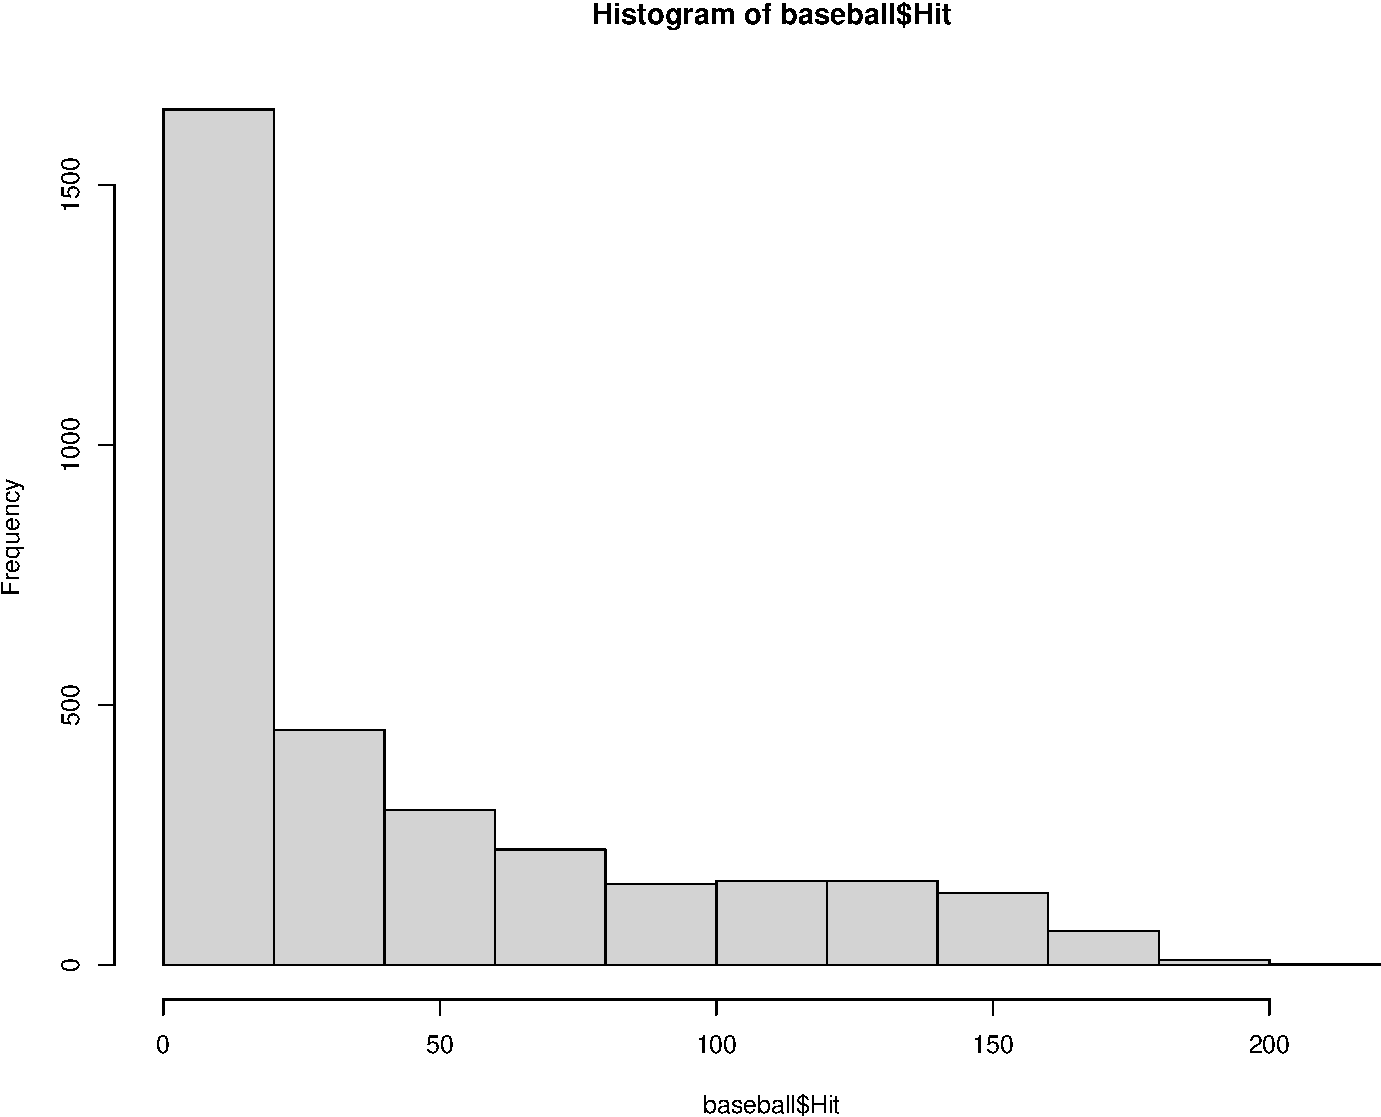
\includegraphics[keepaspectratio]{chap0_introduction_files/figure-pdf/plot1-1.pdf}}

\subsection{可視化してみましょう}\label{ux53efux8996ux5316ux3057ux3066ux307fux307eux3057ux3087ux3046-1}

\begin{itemize}
\tightlist
\item
  \textbf{データは図にする}のが基本です。

  \begin{itemize}
  \tightlist
  \item
    チーム毎のヒット数の違いを見てみましょう
  \item
    ボックスプロット(箱ひげ図)の関数は\texttt{boxplot}です

    \begin{itemize}
    \tightlist
    \item
      x軸がFactor型になっています
    \end{itemize}
  \end{itemize}
\end{itemize}

\begin{Shaded}
\begin{Highlighting}[]
\FunctionTok{boxplot}\NormalTok{(Hit }\SpecialCharTok{\textasciitilde{}}\NormalTok{ team, }\AttributeTok{data =}\NormalTok{ baseball)}
\end{Highlighting}
\end{Shaded}

\pandocbounded{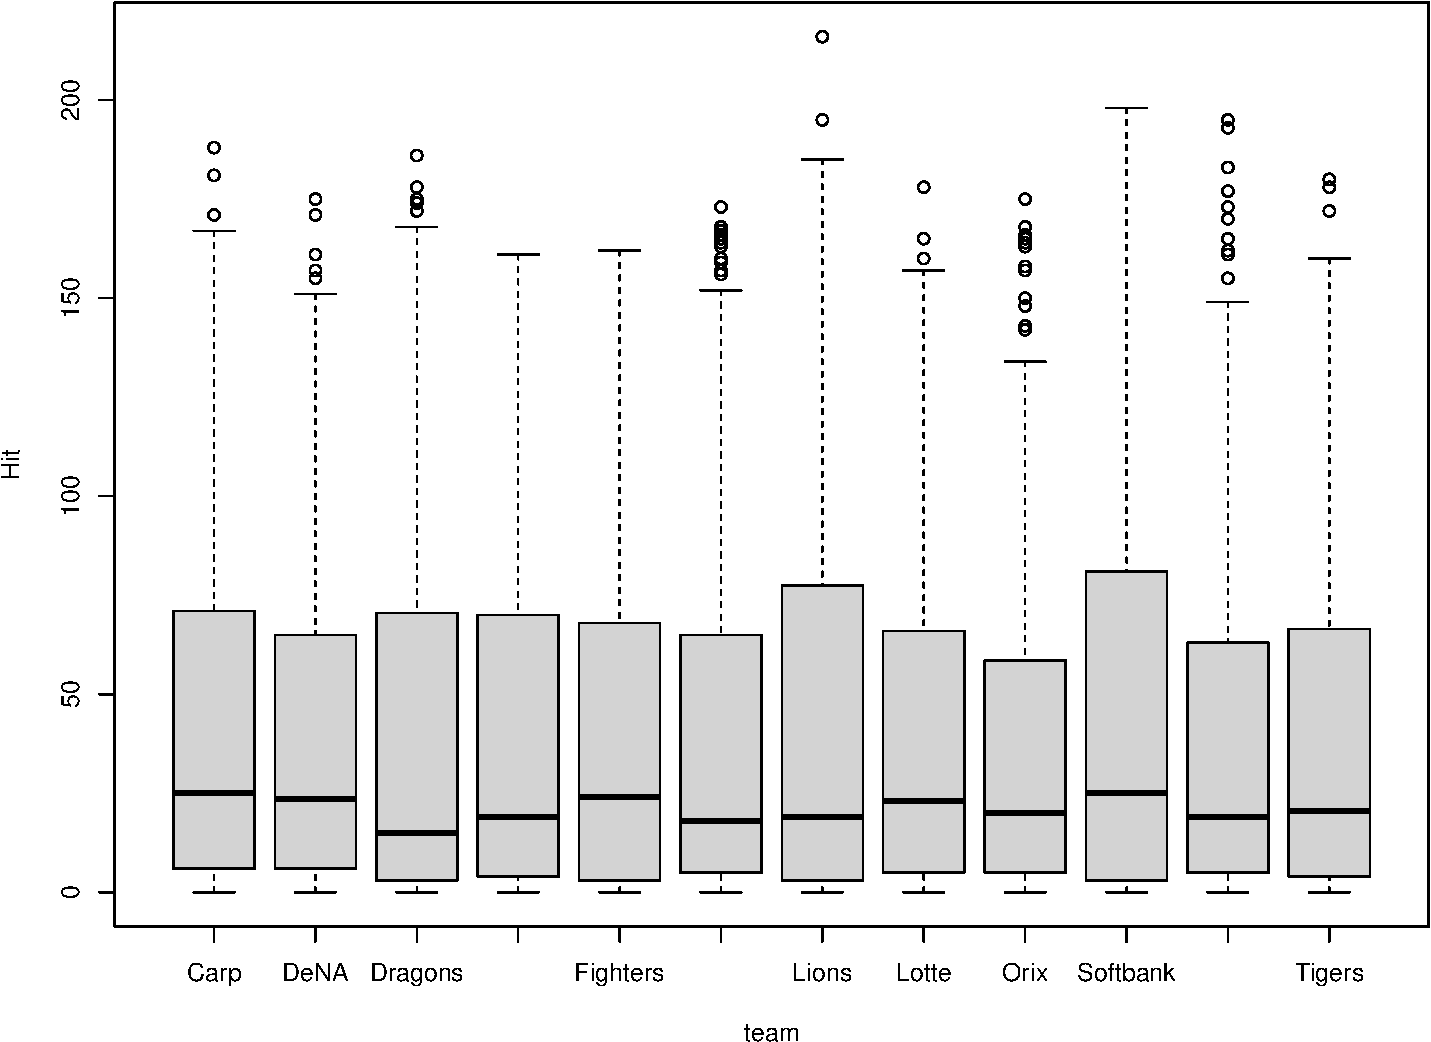
\includegraphics[keepaspectratio]{chap0_introduction_files/figure-pdf/plot2-1.pdf}}

\subsection{可視化してみましょう}\label{ux53efux8996ux5316ux3057ux3066ux307fux307eux3057ux3087ux3046-2}

\begin{itemize}
\tightlist
\item
  \textbf{データは図にする}のが基本です。

  \begin{itemize}
  \tightlist
  \item
    散布図を書いてみましょう
  \item
    散布図は\texttt{plot}関数にx軸とy軸変数を指定します
  \end{itemize}
\end{itemize}

\begin{Shaded}
\begin{Highlighting}[]
\FunctionTok{plot}\NormalTok{(baseball}\SpecialCharTok{$}\NormalTok{height, baseball}\SpecialCharTok{$}\NormalTok{weight)}
\end{Highlighting}
\end{Shaded}

\pandocbounded{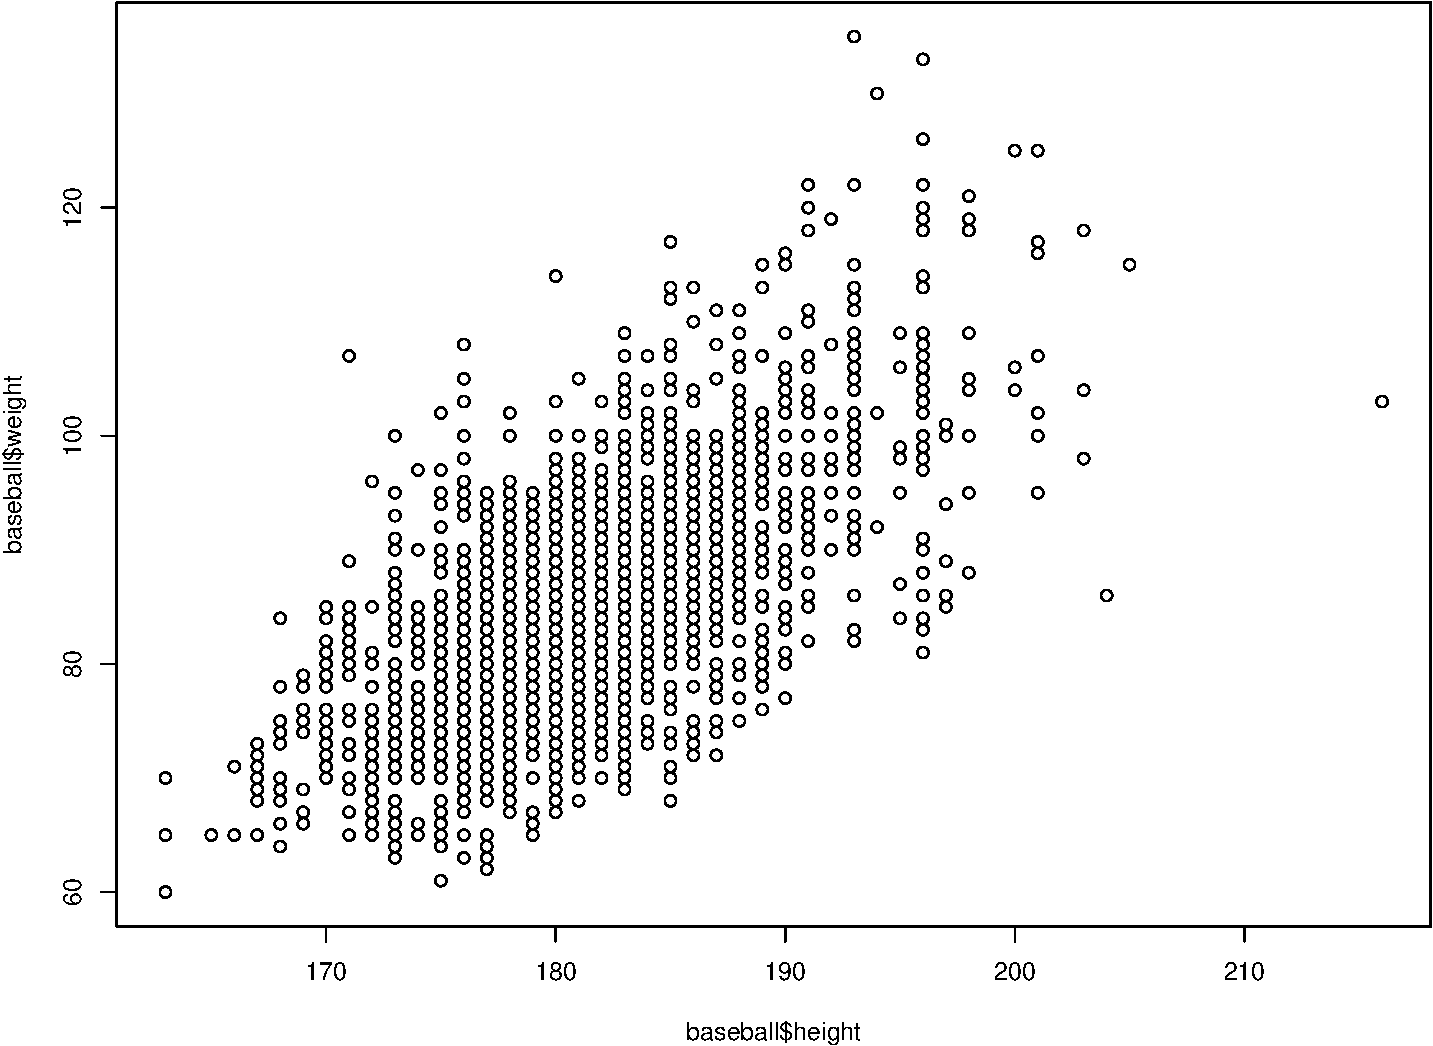
\includegraphics[keepaspectratio]{chap0_introduction_files/figure-pdf/plot3-1.pdf}}

\subsection{(余談)ggplotによる出力は,より綺麗です}\label{ux4f59ux8ac7ggplotux306bux3088ux308bux51faux529bux306fux3088ux308aux7dbaux9e97ux3067ux3059}

\begin{Shaded}
\begin{Highlighting}[]
\FunctionTok{library}\NormalTok{(ggplot2)}
\NormalTok{baseball }\SpecialCharTok{|\textgreater{}}
    \FunctionTok{ggplot}\NormalTok{(}\FunctionTok{aes}\NormalTok{(}\AttributeTok{x =}\NormalTok{ weight, }\AttributeTok{y =}\NormalTok{ height, }\AttributeTok{color =}\NormalTok{ team)) }\SpecialCharTok{+}
    \FunctionTok{geom\_point}\NormalTok{() }\SpecialCharTok{+}
    \FunctionTok{geom\_smooth}\NormalTok{(}\AttributeTok{formula =} \StringTok{"y \textasciitilde{} x"}\NormalTok{, }\AttributeTok{method =} \StringTok{"lm"}\NormalTok{, }\AttributeTok{se =} \ConstantTok{FALSE}\NormalTok{) }\SpecialCharTok{+}
    \FunctionTok{facet\_wrap}\NormalTok{(}\SpecialCharTok{\textasciitilde{}}\NormalTok{team)}
\end{Highlighting}
\end{Shaded}

\pandocbounded{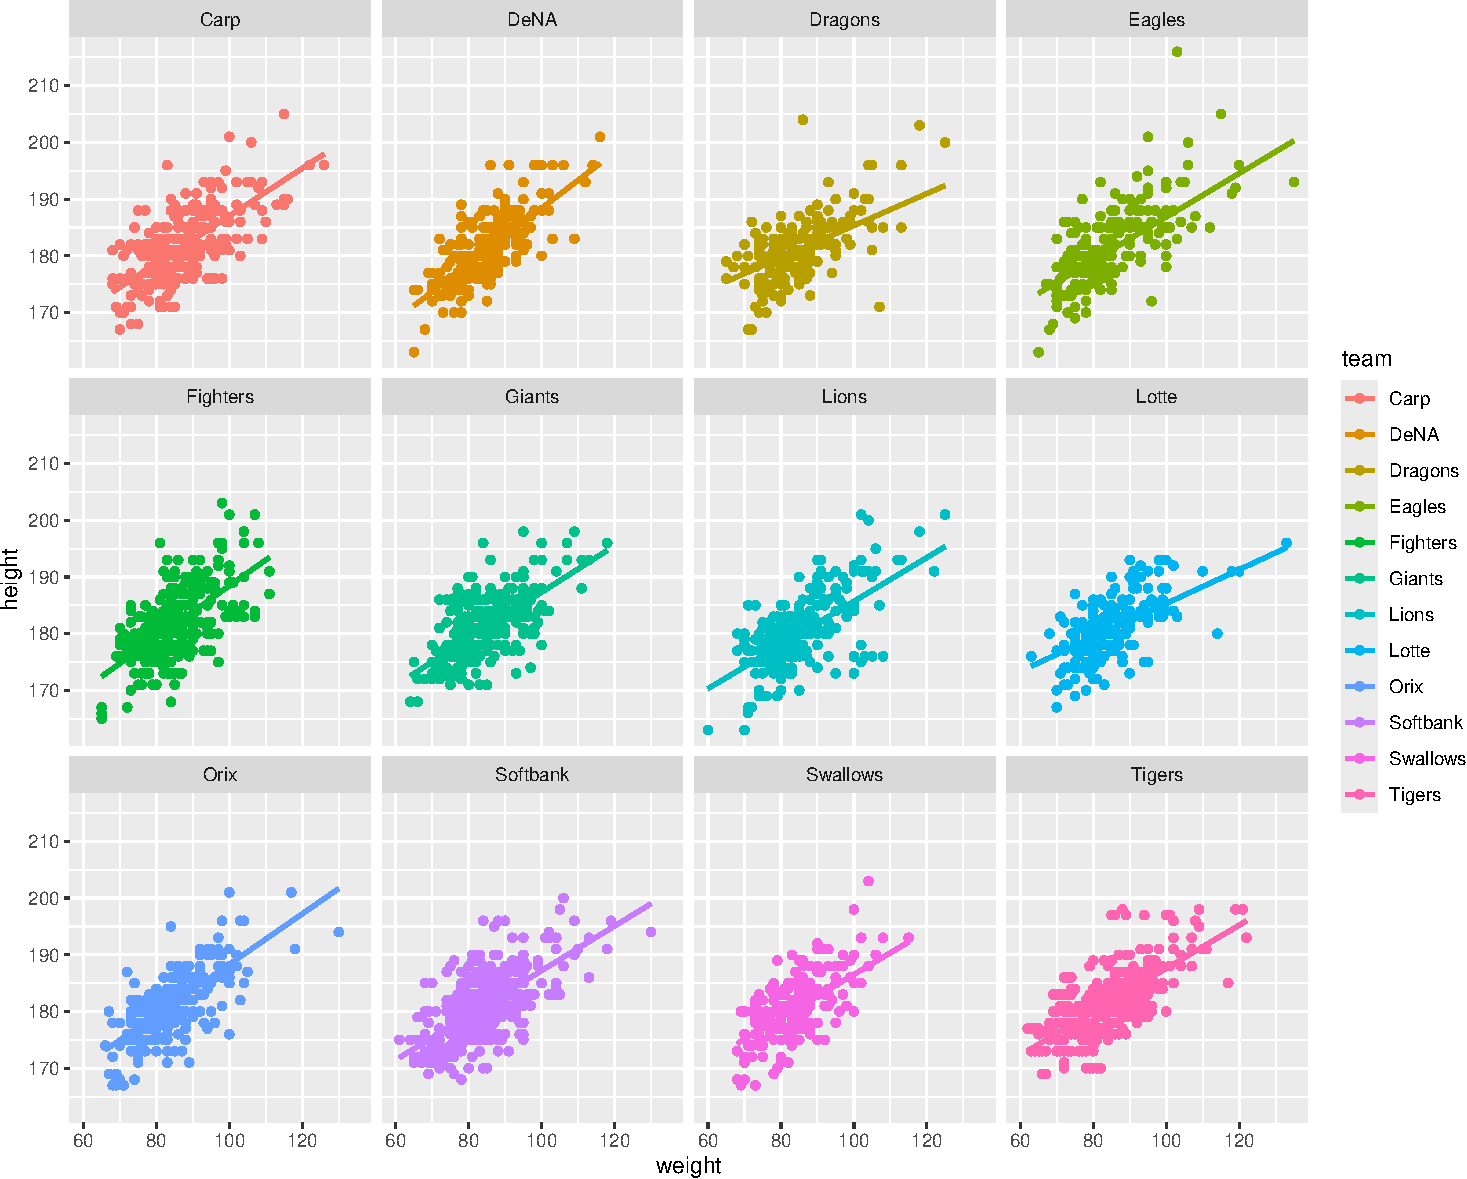
\includegraphics[keepaspectratio]{chap0_introduction_files/figure-pdf/ggplot1-1.pdf}}

\section{Enjoy!}\label{enjoy}

\begin{itemize}
\tightlist
\item
  以上で入門コースは終了です
\item
  この講義では\texttt{exametrika}パッケージの他は,基本的にRの基本関数だけで分析できるようにご案内します。
\item
  実は\texttt{ggexametrika}パッケージというのもあります→\href{https://github.com/kosugitti/ggExametrika}{こちら}
\end{itemize}

\section{Advanced Topics}\label{advanced-topics}

\subsection{Quarto/Rmarkdown:文芸的プログラミング}\label{quartormarkdownux6587ux82b8ux7684ux30d7ux30edux30b0ux30e9ux30dfux30f3ux30b0}

\subsubsection{Rmarkdownとは}\label{rmarkdownux3068ux306f}

\begin{itemize}
\item
  Markdown書式というプレーンな文書作成文法 +
  チャンクと呼ばれるRコードの結合
\item
  文書を作成(レンダリング)するときは,Rの計算を実行してその結果を文書内に反映させる
\item
  コピペ汚染がなく,RStudioで執筆と分析が統合,これだけで完結できます。
\end{itemize}

\subsubsection{Quartoとは}\label{quartoux3068ux306f}

\begin{itemize}
\tightlist
\item
  次世代のR Markdownです。私のスライドもQuartoで作られています
\item
  マルチ言語対応(R, Python, Julia等)
\item
  ePub, PDFなど出力も多様
\end{itemize}

\subsection{Quarto/Rmarkdown:文芸的プログラミング}\label{quartormarkdownux6587ux82b8ux7684ux30d7ux30edux30b0ux30e9ux30dfux30f3ux30b0-1}

\subsubsection{基本的な使い方}\label{ux57faux672cux7684ux306aux4f7fux3044ux65b9-1}

\begin{enumerate}
\def\labelenumi{\arabic{enumi}.}
\tightlist
\item
  File → New FileでQuarto Document / R Markdownを選択
\item
  TitleやAuthorを入力,出力書式(HTML,PDF,Word)などを選ぶ画面が出ます
\item
  サンプル文書・コードが書いてあるファイルが生成されます
\end{enumerate}

これをRneder/Knitすることでファイルが出力されます。




\end{document}
